\chapter{Analyse des Besoins et Conception du Syst\`eme}

\section*{Introduction}
\par Ce troisi\`eme chapitre pr\'esente la d\'emarche rigoureuse d'analyse des exigences et de conception architecturale de notre plateforme. Nous d\'ebutons par l'analyse exhaustive des besoins fonctionnels, non fonctionnels, des contraintes de s\'ecurit\'e et des exigences l\'egales (PoA). Nous formalisons ensuite la mod\'elisation fonctionnelle \`a travers les diagrammes de cas d'utilisation UML. Par la suite, nous d\'etaillons l'architecture globale en distinguant explicitement les \textbf{7 composants applicatifs m\'etier} et les \textbf{12 conteneurs Docker d'infrastructure}. Nous exposons la conception des donn\'ees (mod\`ele relationnel sur 14 tables, diagramme de classes, graphe openCypher, s\'equences d'ex\'ecution, machine \`a \'etats et DFD). Nous d\'eveloppons l'architecture de s\'ecurit\'e multicouche et menons une mod\'elisation formelle des menaces selon la m\'ethodologie STRIDE. Enfin, nous d\'etaillons la cha\^ine DevSecOps int\'egr\'ee au pipeline de livraison logicielle.

\section{Analyse des Besoins}
\subsection{Identification des Acteurs}
\par Le syst\`eme interagit avec quatre profils d'acteurs op\'erationnels distincts :
\begin{itemize}
    \item \textbf{L'Analyste de S\'ecurit\'e (Security Analyst) :} Utilisateur op\'erationnel principal qui configure les cibles d'audit, t\'el\'everse les preuves d'autorisation (PoA), lance les scans, analyse les r\'esultats techniques, explore le graphe de connaissances, valide les scripts de rem\'ediation IA et exporte les rapports d'expertise.
    \item \textbf{Le Client / Lecteur (Client / Viewer) :} B\'en\'eficiaire des audits, consultant en lecture seule les tableaux de bord synth\'etiques, les rapports valid\'es et acquittant les alertes de s\'ecurit\'e li\'ees \`a son p\'erim\`etre d'actifs.
    \item \textbf{L'Administrateur Syst\`eme (System Administrator) :} Supervise la gouvernance globale de la plateforme, la gestion des comptes utilisateurs, l'attribution des r\^oles RBAC, la configuration des quotas de scan et la surveillance de l'\'etat de sant\'e des microservices conteneuris\'es.
    \item \textbf{L'Auditeur / Responsable Conformit\'e (Auditor / Compliance) :} Profil d\'edi\'e au contr\^ole r\'eglementaire, consultant en lecture seule les journaux d'audit immuables (\textit{Audit Logs}), contr\^olant la validit\'e juridique des mandats PoA et v\'erifiant la tra\c{c}abilit\'e exhaustive de l'ensemble des actions men\'ees.
\end{itemize}
\par \textit{Remarque :} Le Responsable Technique (CTO) de l'entreprise d'accueil assure l'encadrement industriel, la revue d'architecture et la gouvernance globale du projet, sans constituer un acteur op\'erationnel direct au sens de la mod\'elisation UML du syst\`eme.

\subsection{Besoins Fonctionnels}
\par Conform\'ement au cahier des charges valid\'e avec Designet Web Agency, les besoins fonctionnels prioritaires couvrent :
\begin{itemize}
    \item \textbf{Gestion des Cibles et Mandats :} Enregistrement s\'ecuris\'e des cibles d'audit (domaines, sous-domaines, plages IP) avec t\'el\'eversement et validation obligatoire d'une preuve d'autorisation (PoA).
    \item \textbf{Orchestration des Scans :} Configuration et d\'eclenchement asynchrone des scanners (Nmap, Nuclei, Gobuster, Subfinder, WPScan) selon 3 profils d'intensit\'e (Silent, Balanced, Aggressive) avec gestion du jitter anti-blocage.
    \item \textbf{Normalisation des Constats :} Transformation automatique des sorties brutes h\'et\'erog\`enes en entit\'es normalis\'ees \textit{Finding} avec score de s\'ev\'erit\'e, mapping CVE/CWE et citations des num\'eros de lignes de logs bruts.
    \item \textbf{Mod\'elisation en Graphe de Connaissances :} Projection de la topologie de la cible sous forme de graphe relationnel avec calcul du rayon d'impact (\textit{blast radius}) par l'algorithme BFS sous NetworkX.
    \item \textbf{Assistance IA et Remediation-as-Code :} G\'en\'eration automatis\'ee de synth\`eses manag\'eriales et de scripts durcis de correction (Bash, Ansible, Dockerfile, Terraform) via un mod\`ele de langage local contraint.
    \item \textbf{Modules de S\'ecurit\'e Offensive et Sandbox :} Tests d'injection (SQL, commandes, XSS), analyse de WAF et d\'eploiement \`a la demande d'environnements vuln\'erables isol\'es (DVWA, SQLi-Labs, WebGoat, bWAPP).
    \item \textbf{G\'en\'eration et Export de Rapports :} Production de rapports d'audit complets aux formats PDF sign\'e, HTML et JSON, avec m\'ecanisme de partage par liens temporaires s\'ecuris\'es.
\end{itemize}

\subsection{Besoins Non Fonctionnels}
\begin{itemize}
    \item \textbf{S\'ecurit\'e \& Confidentialit\'e :} Application du principe de moindre privil\`ege, conteneurs non-root (UID 1001), syst\`eme de fichiers en lecture seule, chiffrement des secrets et terminaison TLS 1.3.
    \item \textbf{Scalabilit\'e \& R\'esilience :} D\'ecouplage des t\^aches lourdes par files Redis Streams avec r\'eessais automatiques et repli exponentiel.
    \item \textbf{Performance :} Temps de r\'eponse de l'interface inf\'erieur \`a 200 ms (P95) pour les pages du tableau de bord.
    \item \textbf{Maintenabilit\'e :} Standardisation des microservices via la classe abstraite \texttt{BaseScannerService} et documentation compl\`ete des endpoints REST.
\end{itemize}

\subsection{Contraintes et Exigences de S\'ecurit\'e}
\par La plateforme manipule des outils et des informations hautement sensibles. Elle impose par cons\'equent une isolation herm\'etique des processus d'audit, l'interdiction stricte de toute action de d\'efacement ou de d\'eni de service, et une journalisation infalsifiable de toutes les requ\^etes administratives.

\subsection{Contraintes L\'egales et Preuve d'Autorisation (Proof of Authorization -- PoA)}
\par L'ex\'ecution d'activit\'es de reconnaissance offensive sur des syst\`emes d'information est strictement encadr\'ee par la l\'egislation (Code P\'enal tunisien, Convention de Budapest, r\'eglementations internationales). Afin de renforcer la conformit\'e l\'egale et \'ethique, notre plateforme impl\'emente une barri\`ere bloquante logicielle : aucun scan de reconnaissance actif ne peut \^etre lanc\'e sans qu'un document de preuve d'autorisation (PoA) valide, d\^ument sign\'e par le propri\'etaire de la cible, ne soit attach\'e et valid\'e dans le projet.

\section{Mod\'elisation Fonctionnelle UML}
\subsection{Diagramme Global des Cas d'Utilisation}
\par Le diagramme global mod\'elise l'ensemble des cas d'utilisation structur\'es selon les quatre r\^oles du syst\`eme.

\begin{figure}[!htbp]
    \centering
    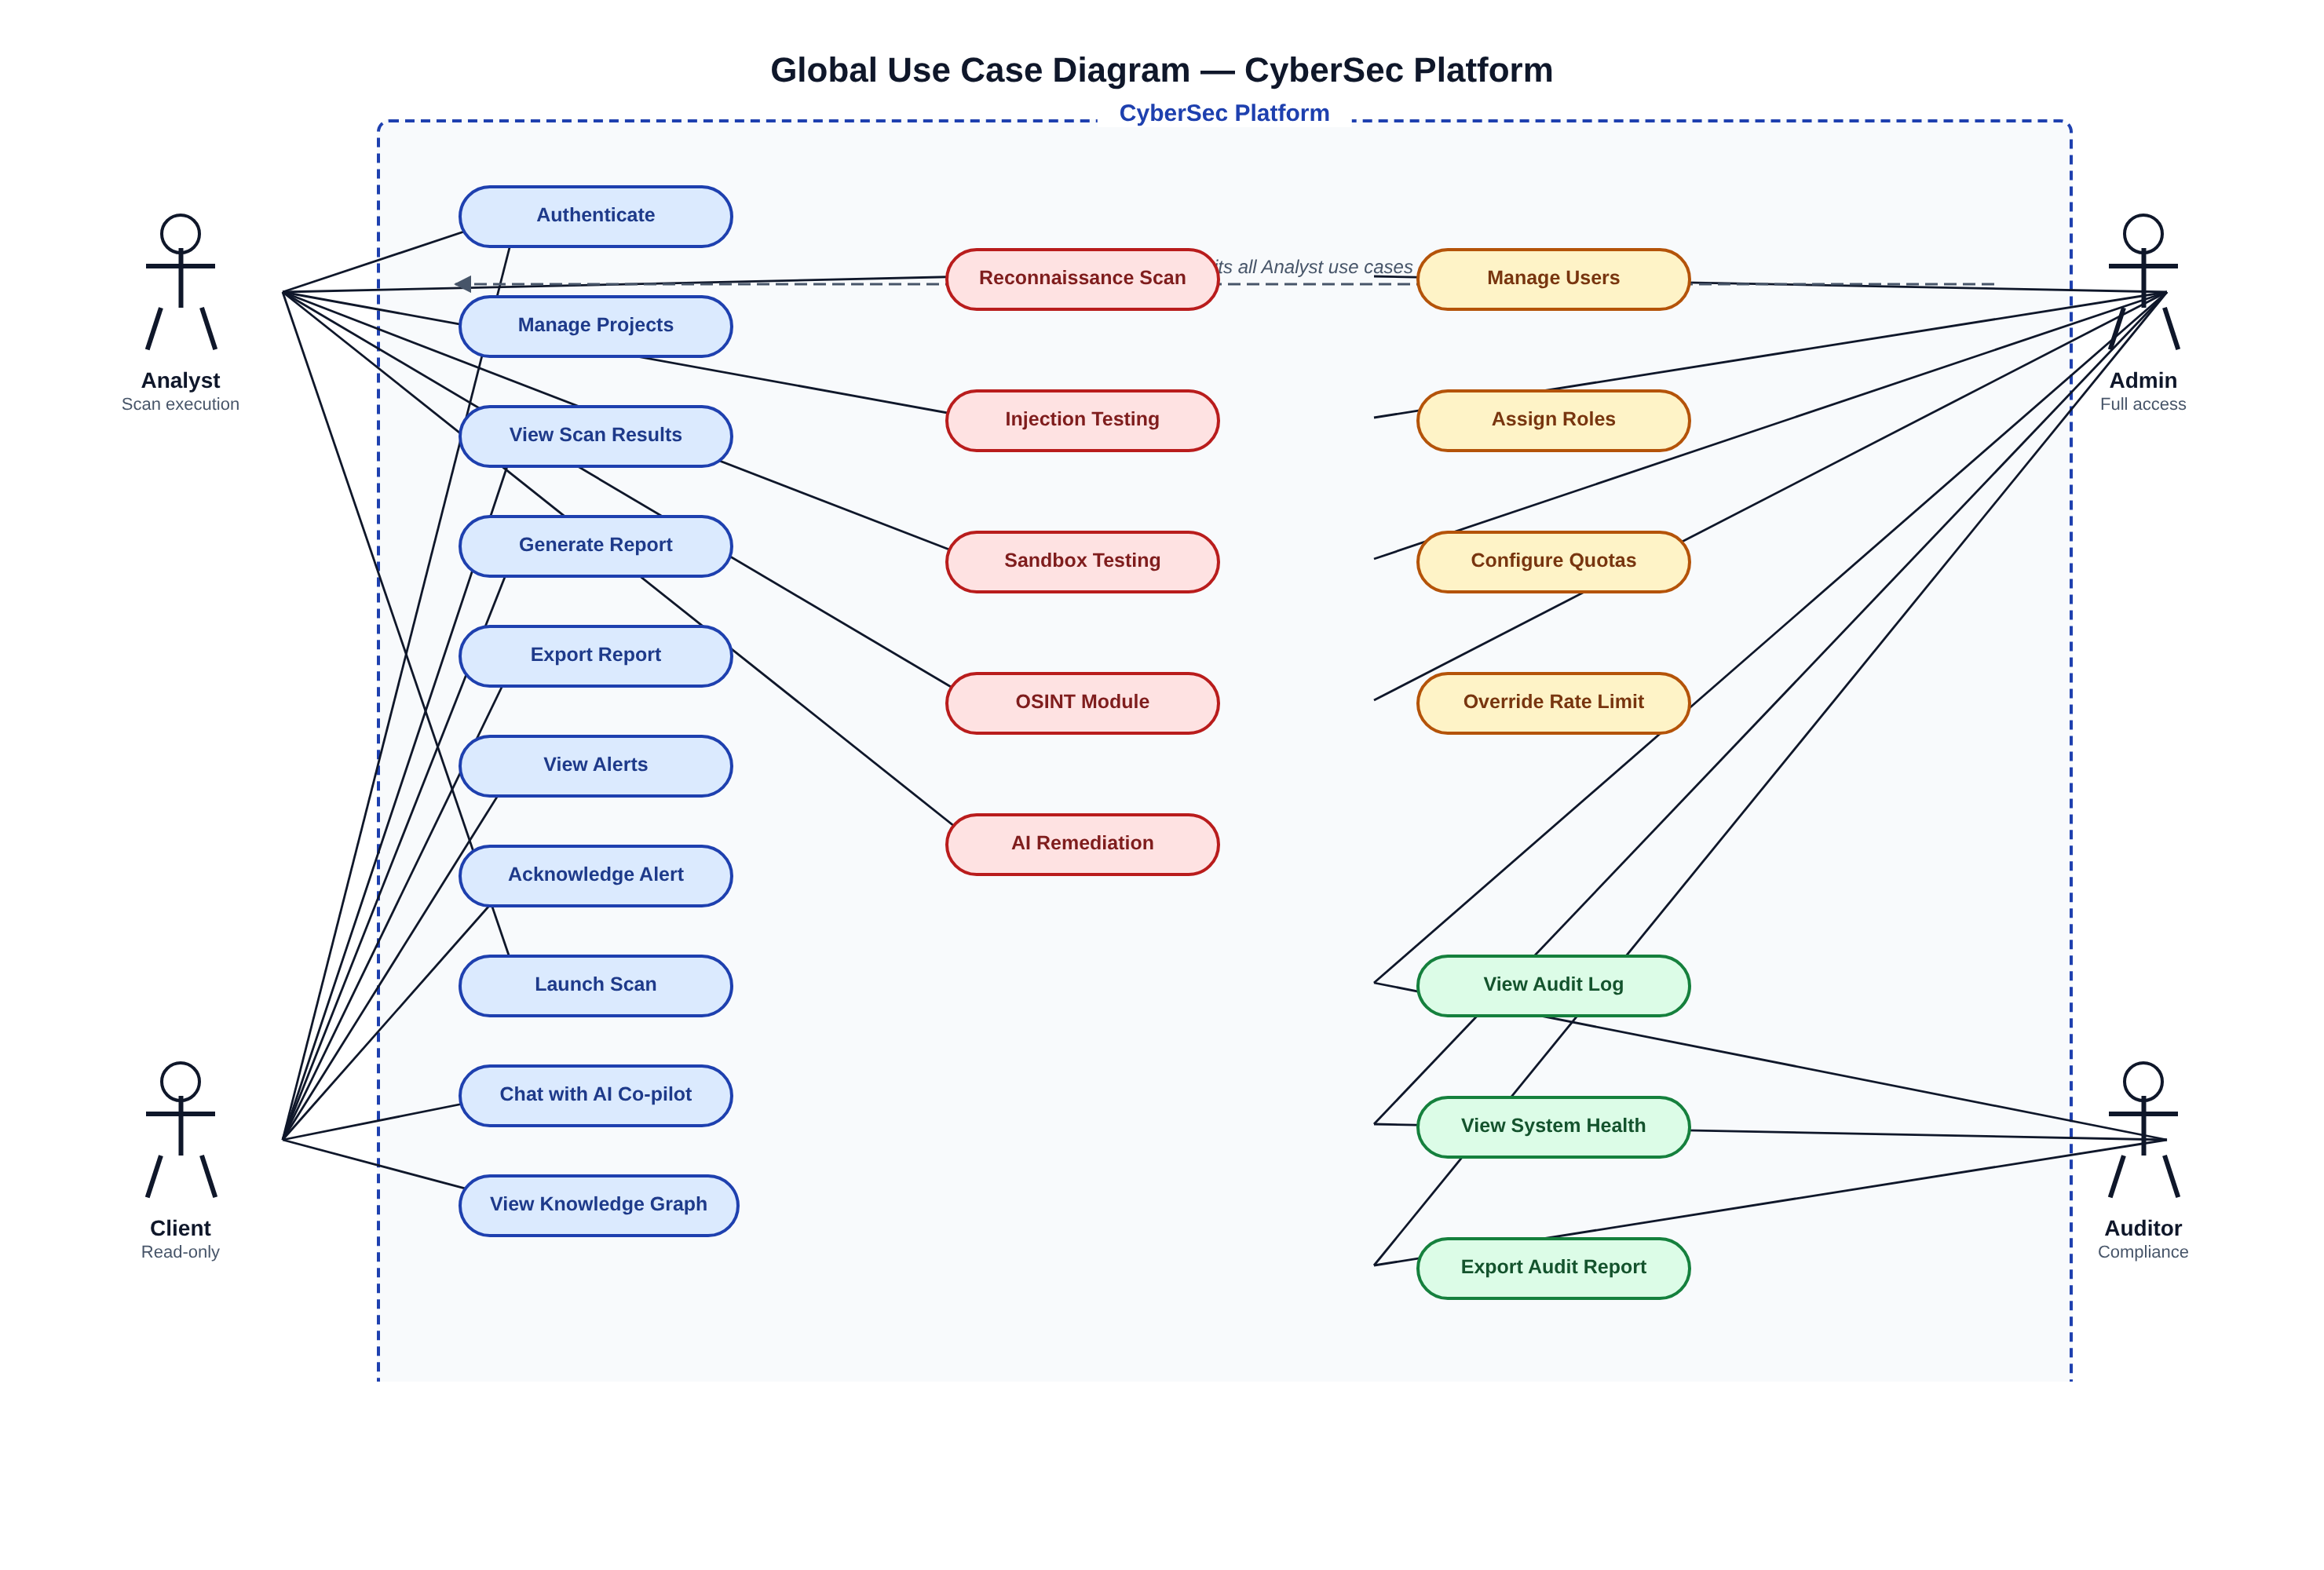
\includegraphics[width=0.82\textwidth]{img/usecase_global.png}
    \caption{Diagramme Global des Cas d'Utilisation -- Acteurs et Fonctionnalit\'es Cl\'es}
    \label{fig:usecase_global}
\end{figure}

\subsection{Cas d'Utilisation de l'Analyste de S\'ecurit\'e}
\par L'analyste configure les audits, explore les r\'esultats, manipule le graphe et valide les rem\'ediations.

\begin{figure}[!htbp]
    \centering
    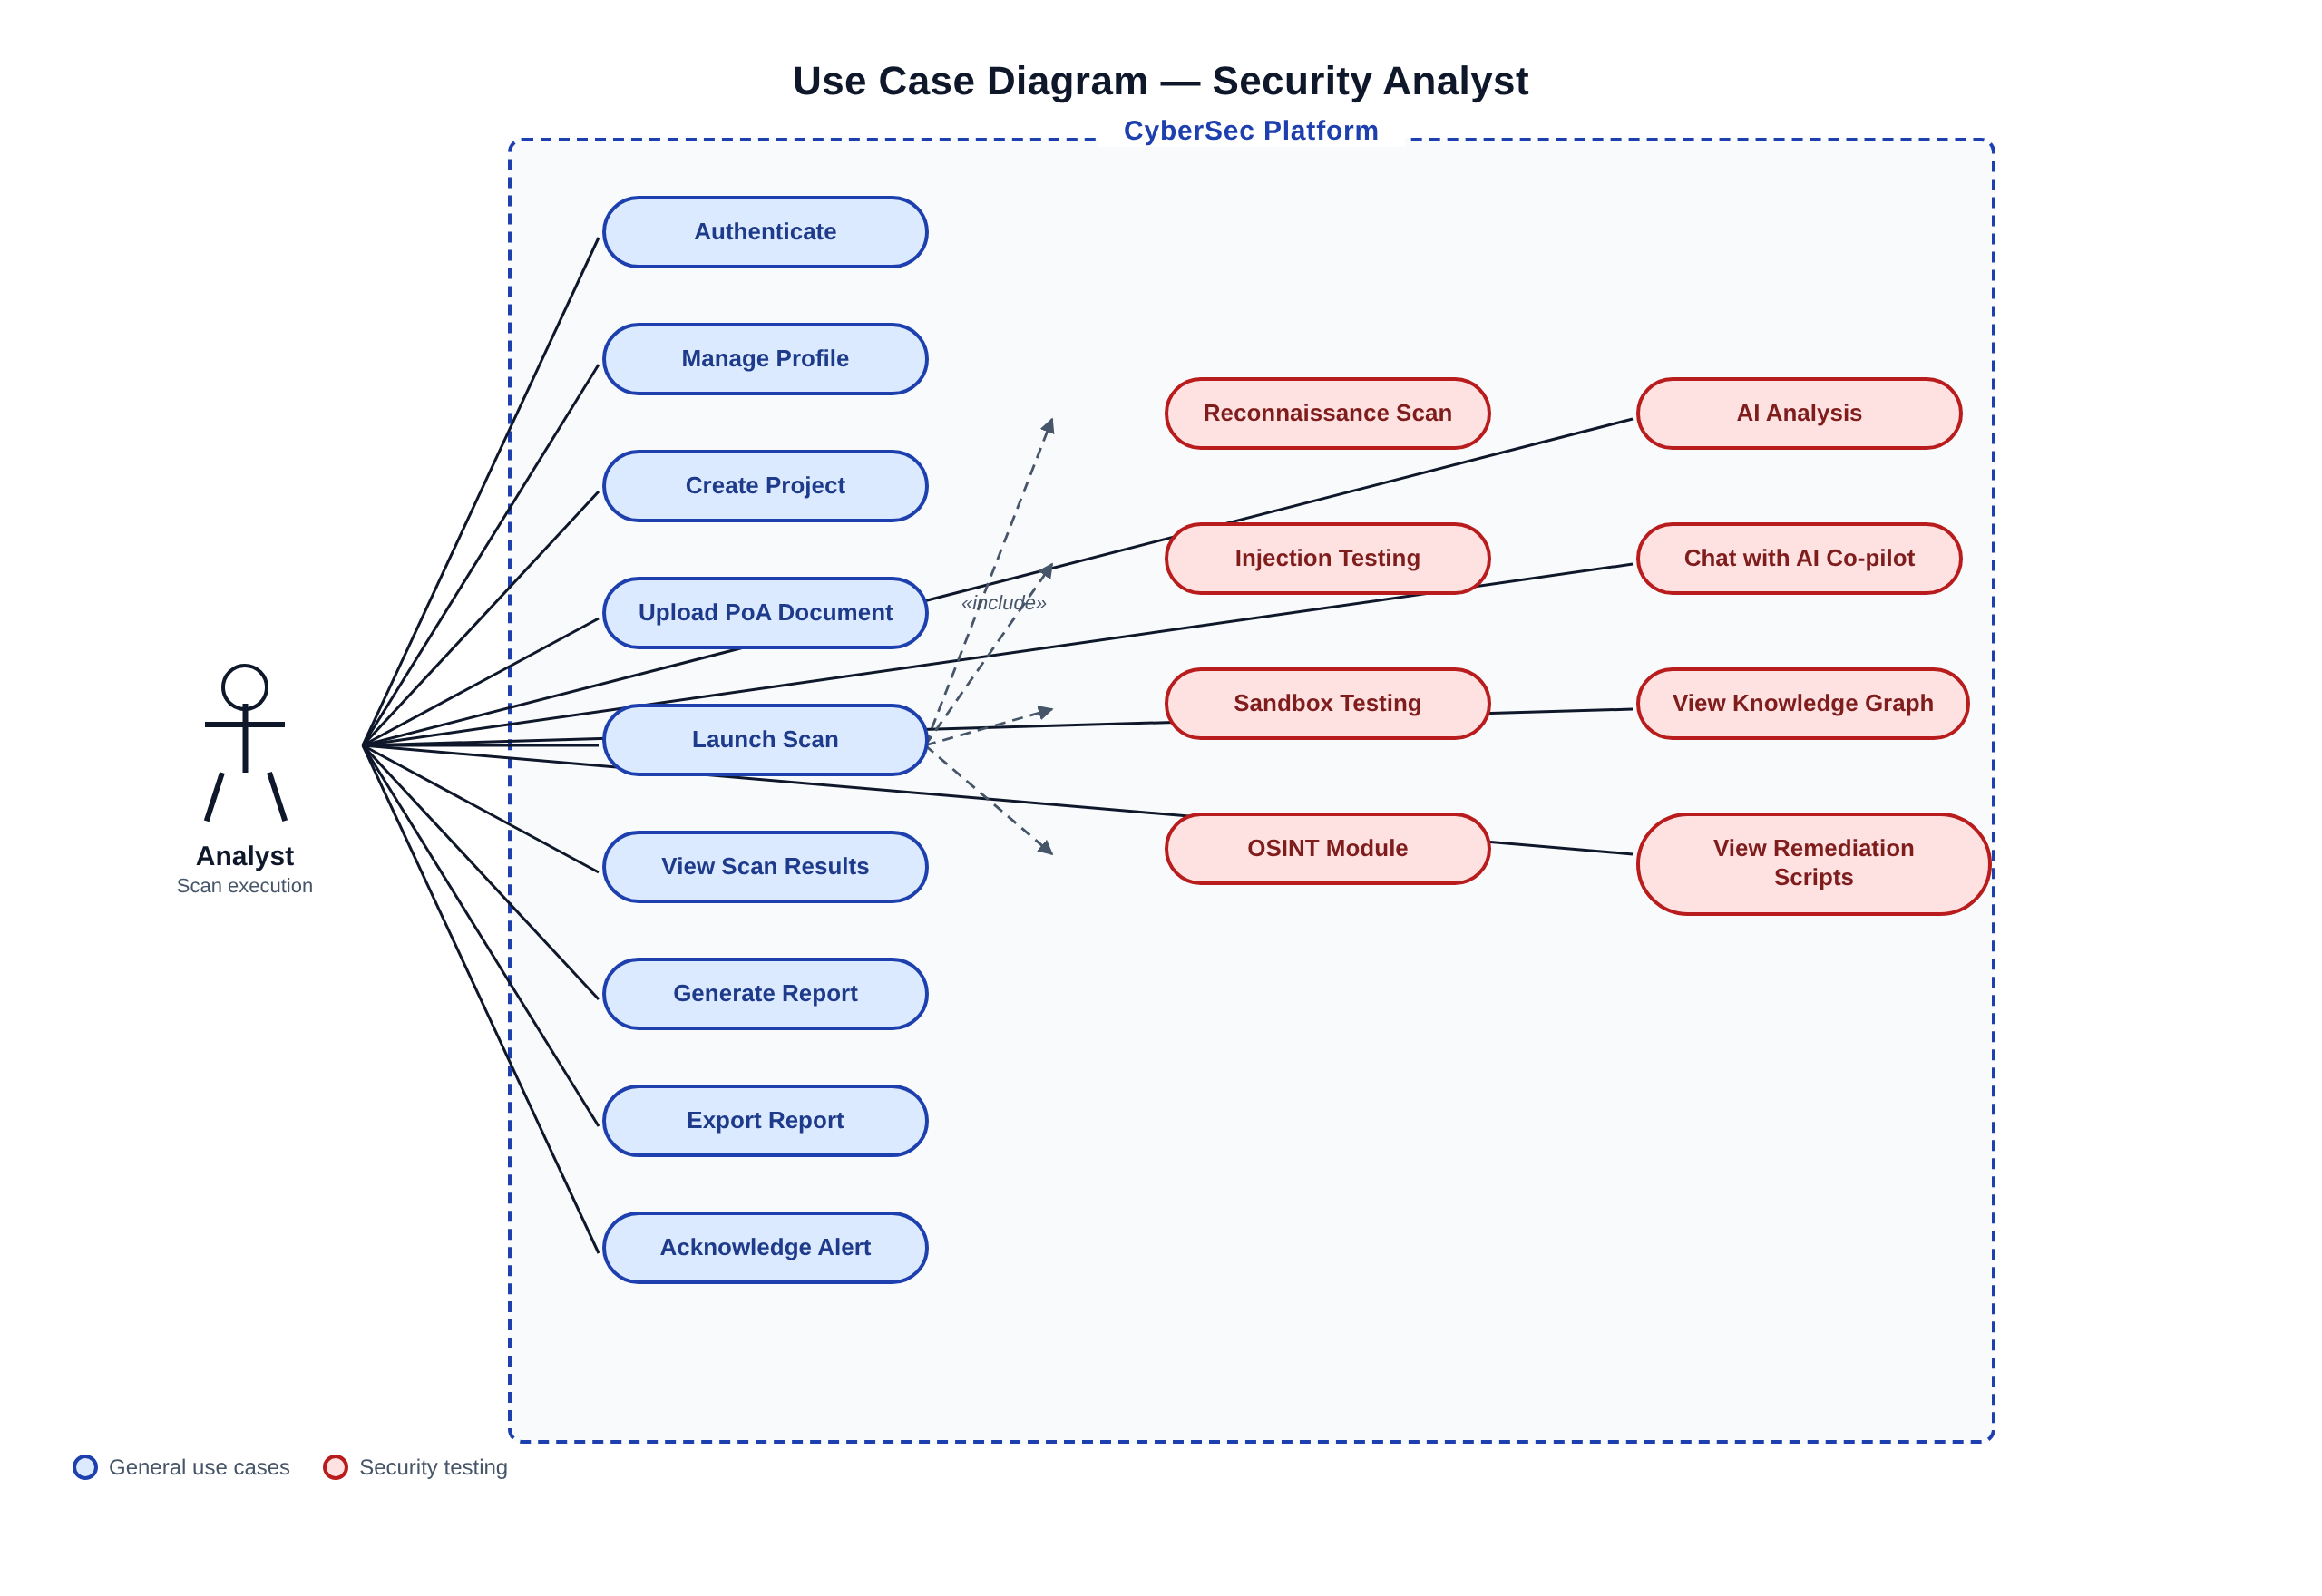
\includegraphics[width=0.82\textwidth]{img/usecase_analyst.png}
    \caption{Diagramme des Cas d'Utilisation -- Analyste de S\'ecurit\'e}
    \label{fig:usecase_analyst}
\end{figure}

\subsection{Cas d'Utilisation de l'Administrateur Syst\`eme}
\par L'administrateur g\`ere les privil\`eges, supervise la sant\'e des microservices et contr\^ole les pistes d'audit.

\begin{figure}[!htbp]
    \centering
    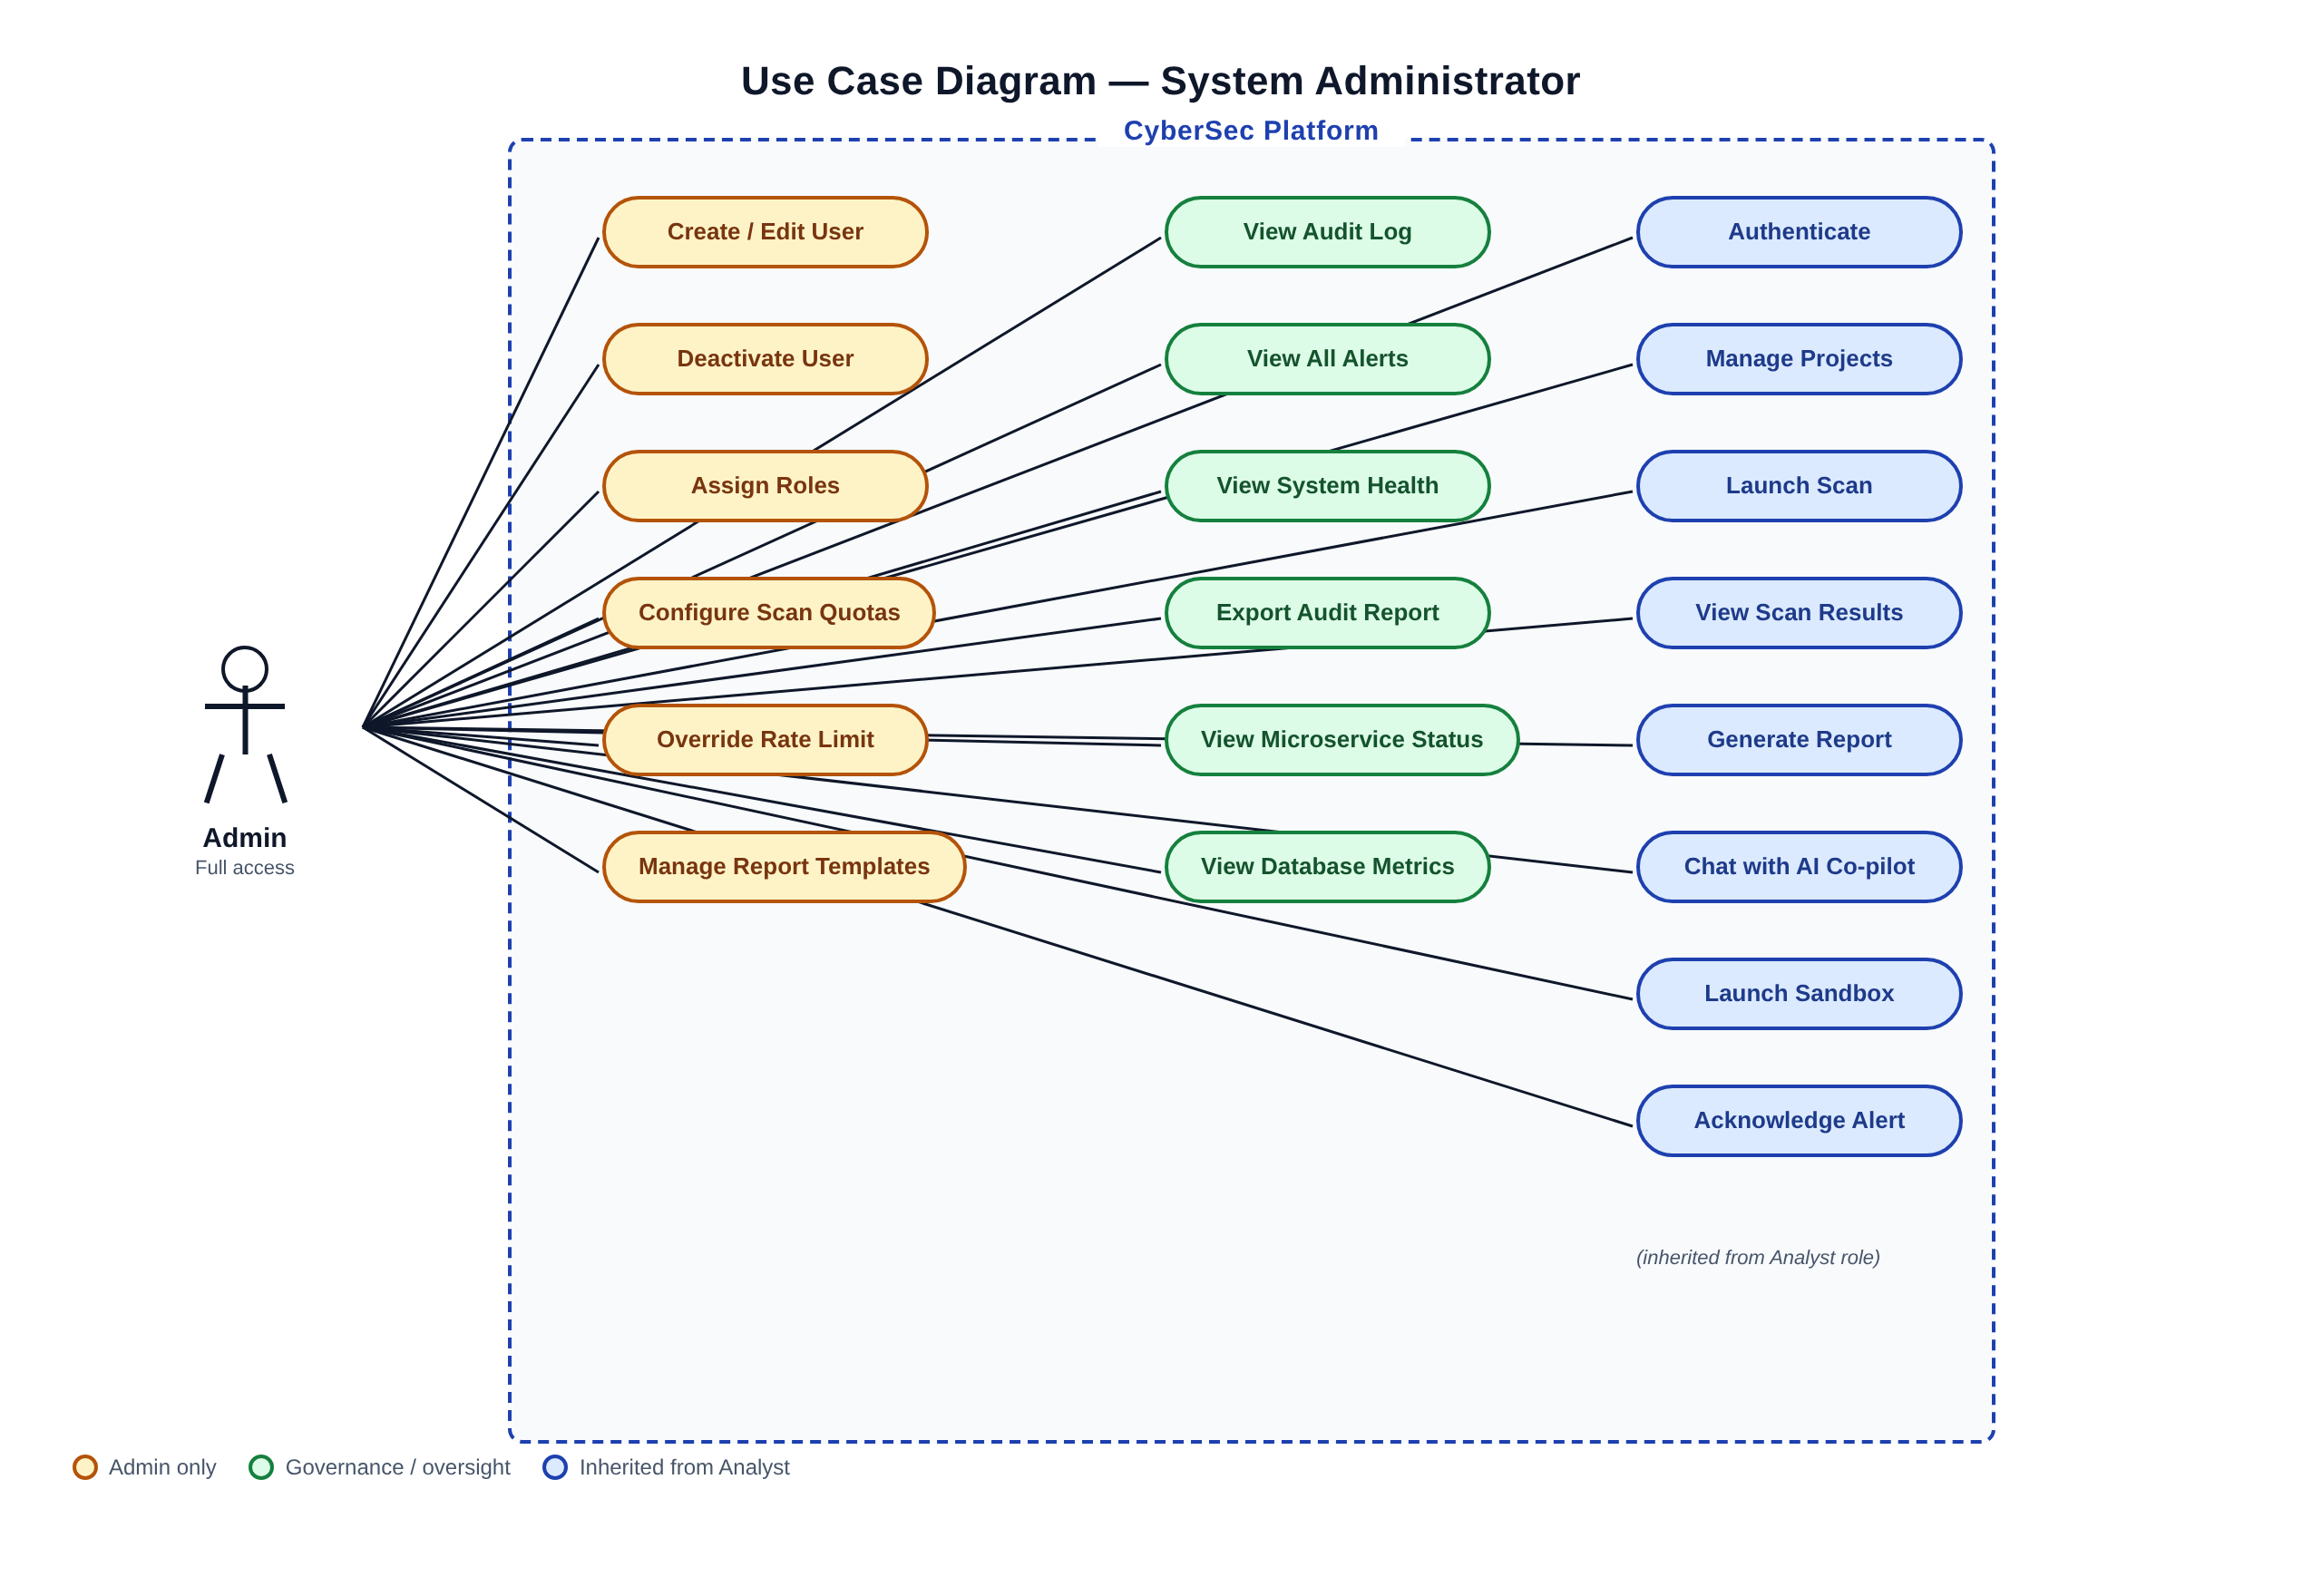
\includegraphics[width=0.82\textwidth]{img/usecase_admin.png}
    \caption{Diagramme des Cas d'Utilisation -- Administrateur Syst\`eme}
    \label{fig:usecase_admin}
\end{figure}

\subsection{Description Textuelle des Principaux Cas d'Utilisation}
\par \textbf{CU01 -- Lancement d'un Scan d'Audit :} L'analyste s\'electionne un projet et une cible, choisit le profil d'intensit\'e (Silent, Balanced, Aggressive), valide la pr\'esence de la PoA, et soumet la requ\^ete. Le back-end ins\`ere la commande dans Redis Streams et retourne un identifiant de session.
\par \textbf{CU02 -- G\'en\'eration de Remediation-as-Code :} L'analyste consulte un constat de vuln\'erabilit\'e et sollicite l'IA. Le microservice transmet le contexte technique \`a Ollama, r\'ecup\`ere le script structur\'e (Bash, Ansible, Dockerfile, Terraform) et l'affiche avec ses citations directes vers les logs bruts.

\section{Architecture Globale du Syst\`eme}
\subsection{Vue d'Ensemble du Syst\`eme}
\par La plateforme adopte une architecture microservices distribu\'ee et segment\'ee, assurant une s\'eparation nette des responsabilit\'es, une meilleure r\'esilience et une s\'ecurit\'e renforc\'ee par conception.

\subsection{Composants Applicatifs M\'etier (7 Composants Logiques)}
\par Sur le plan fonctionnel, l'application est r\'epartie en sept composants logiciels autonomes :
\begin{enumerate}
    \item \textbf{Back-end Web Applicatif (Laravel 11, Port 8000) :} Portail principal, gestion de l'authentification Sanctum, contr\^ole RBAC Spatie, mod\`ele ORM Eloquent, rendu des vues Blade et distribution des t\^aches vers les files de messages.
    \item \textbf{Microservice de Reconnaissance (Flask, Port 5000) :} Moteur d'ex\'ecution des scanners Nmap, Nuclei, Gobuster, Subfinder et WPScan, normalisation des r\'esultats (\texttt{ResultParser}) et initialisation de la topologie de graphe.
    \item \textbf{Microservice de S\'ecurit\'e Offensive (Flask, Port 5001) :} Modules d'\'evaluation des injections SQL/commandes/XSS, analyse de WAF et pilotage s\'ecuris\'e des bacs \`a sable conteneuris\'es.
    \item \textbf{Microservice OSINT (Flask, Port 5002) :} Renseignement passif (enregistrements DNS, requ\^etes WHOIS, certificats SSL/TLS via \texttt{crt.sh}, d\'etection d'empreintes technologiques).
    \item \textbf{Microservice d'IA Contrainte (Flask, Port 5003) :} Couche d'assistance intelligente connect\'ee au mod\`ele local \texttt{qwen2.5-coder} via Ollama pour la production de Remediation-as-Code.
    \item \textbf{Passerelle d'API (API Gateway, Flask, Port 8080) :} Point d'entr\'ee et routeur interne vers les microservices, assurant le contr\^ole de d\'ebit (\textit{rate limiting}) et la tra\c{c}abilit\'e par \texttt{X-Correlation-ID}.
    \item \textbf{Worker Asynchrone (Python) :} Processus d'arri\`ere-plan consommant les \'ev\'enements de scan via \texttt{XREADGROUP} sur Redis Streams, coordonnant les t\^aches longues et persistant les constats dans PostgreSQL.
\end{enumerate}

\subsection{Conteneurs d'Infrastructure Docker (12 Services Conteneuris\'es)}
\par Sur le plan infrastructurel, le d\'eploiement orchestre douze conteneurs Docker compl\'ementaires :
\begin{itemize}
    \item Les 7 conteneurs h\'ebergeant les 7 composants applicatifs d\'ecrits ci-dessus.
    \item \textbf{8. Nginx 1.27 :} Serveur mandataire inverse (\textit{reverse proxy}) assurant la terminaison TLS 1.3 et le durcissement des en-t\^etes HTTP.
    \item \textbf{9. PostgreSQL 16 + Apache AGE :} Syst\`eme de gestion de base de donn\'ees unifi\'e relationnel (14 tables) et graphe openCypher.
    \item \textbf{10. Redis 7 :} Magasin de donn\'ees en m\'emoire servant de Message Broker Streams, cache applicatif et gestionnaire de sessions.
    \item \textbf{11. Ollama :} Serveur d'inf\'erence local ex\'ecutant le mod\`ele d\'edi\'e au code \texttt{qwen2.5-coder}.
    \item \textbf{12. Docker-Socket-Proxy :} Proxy de s\'ecurit\'e interdisant les acc\`es directs au socket Unix de Docker pour pr\'evenir toute \'evasion de conteneur.
\end{itemize}

\begin{figure}[!htbp]
    \centering
    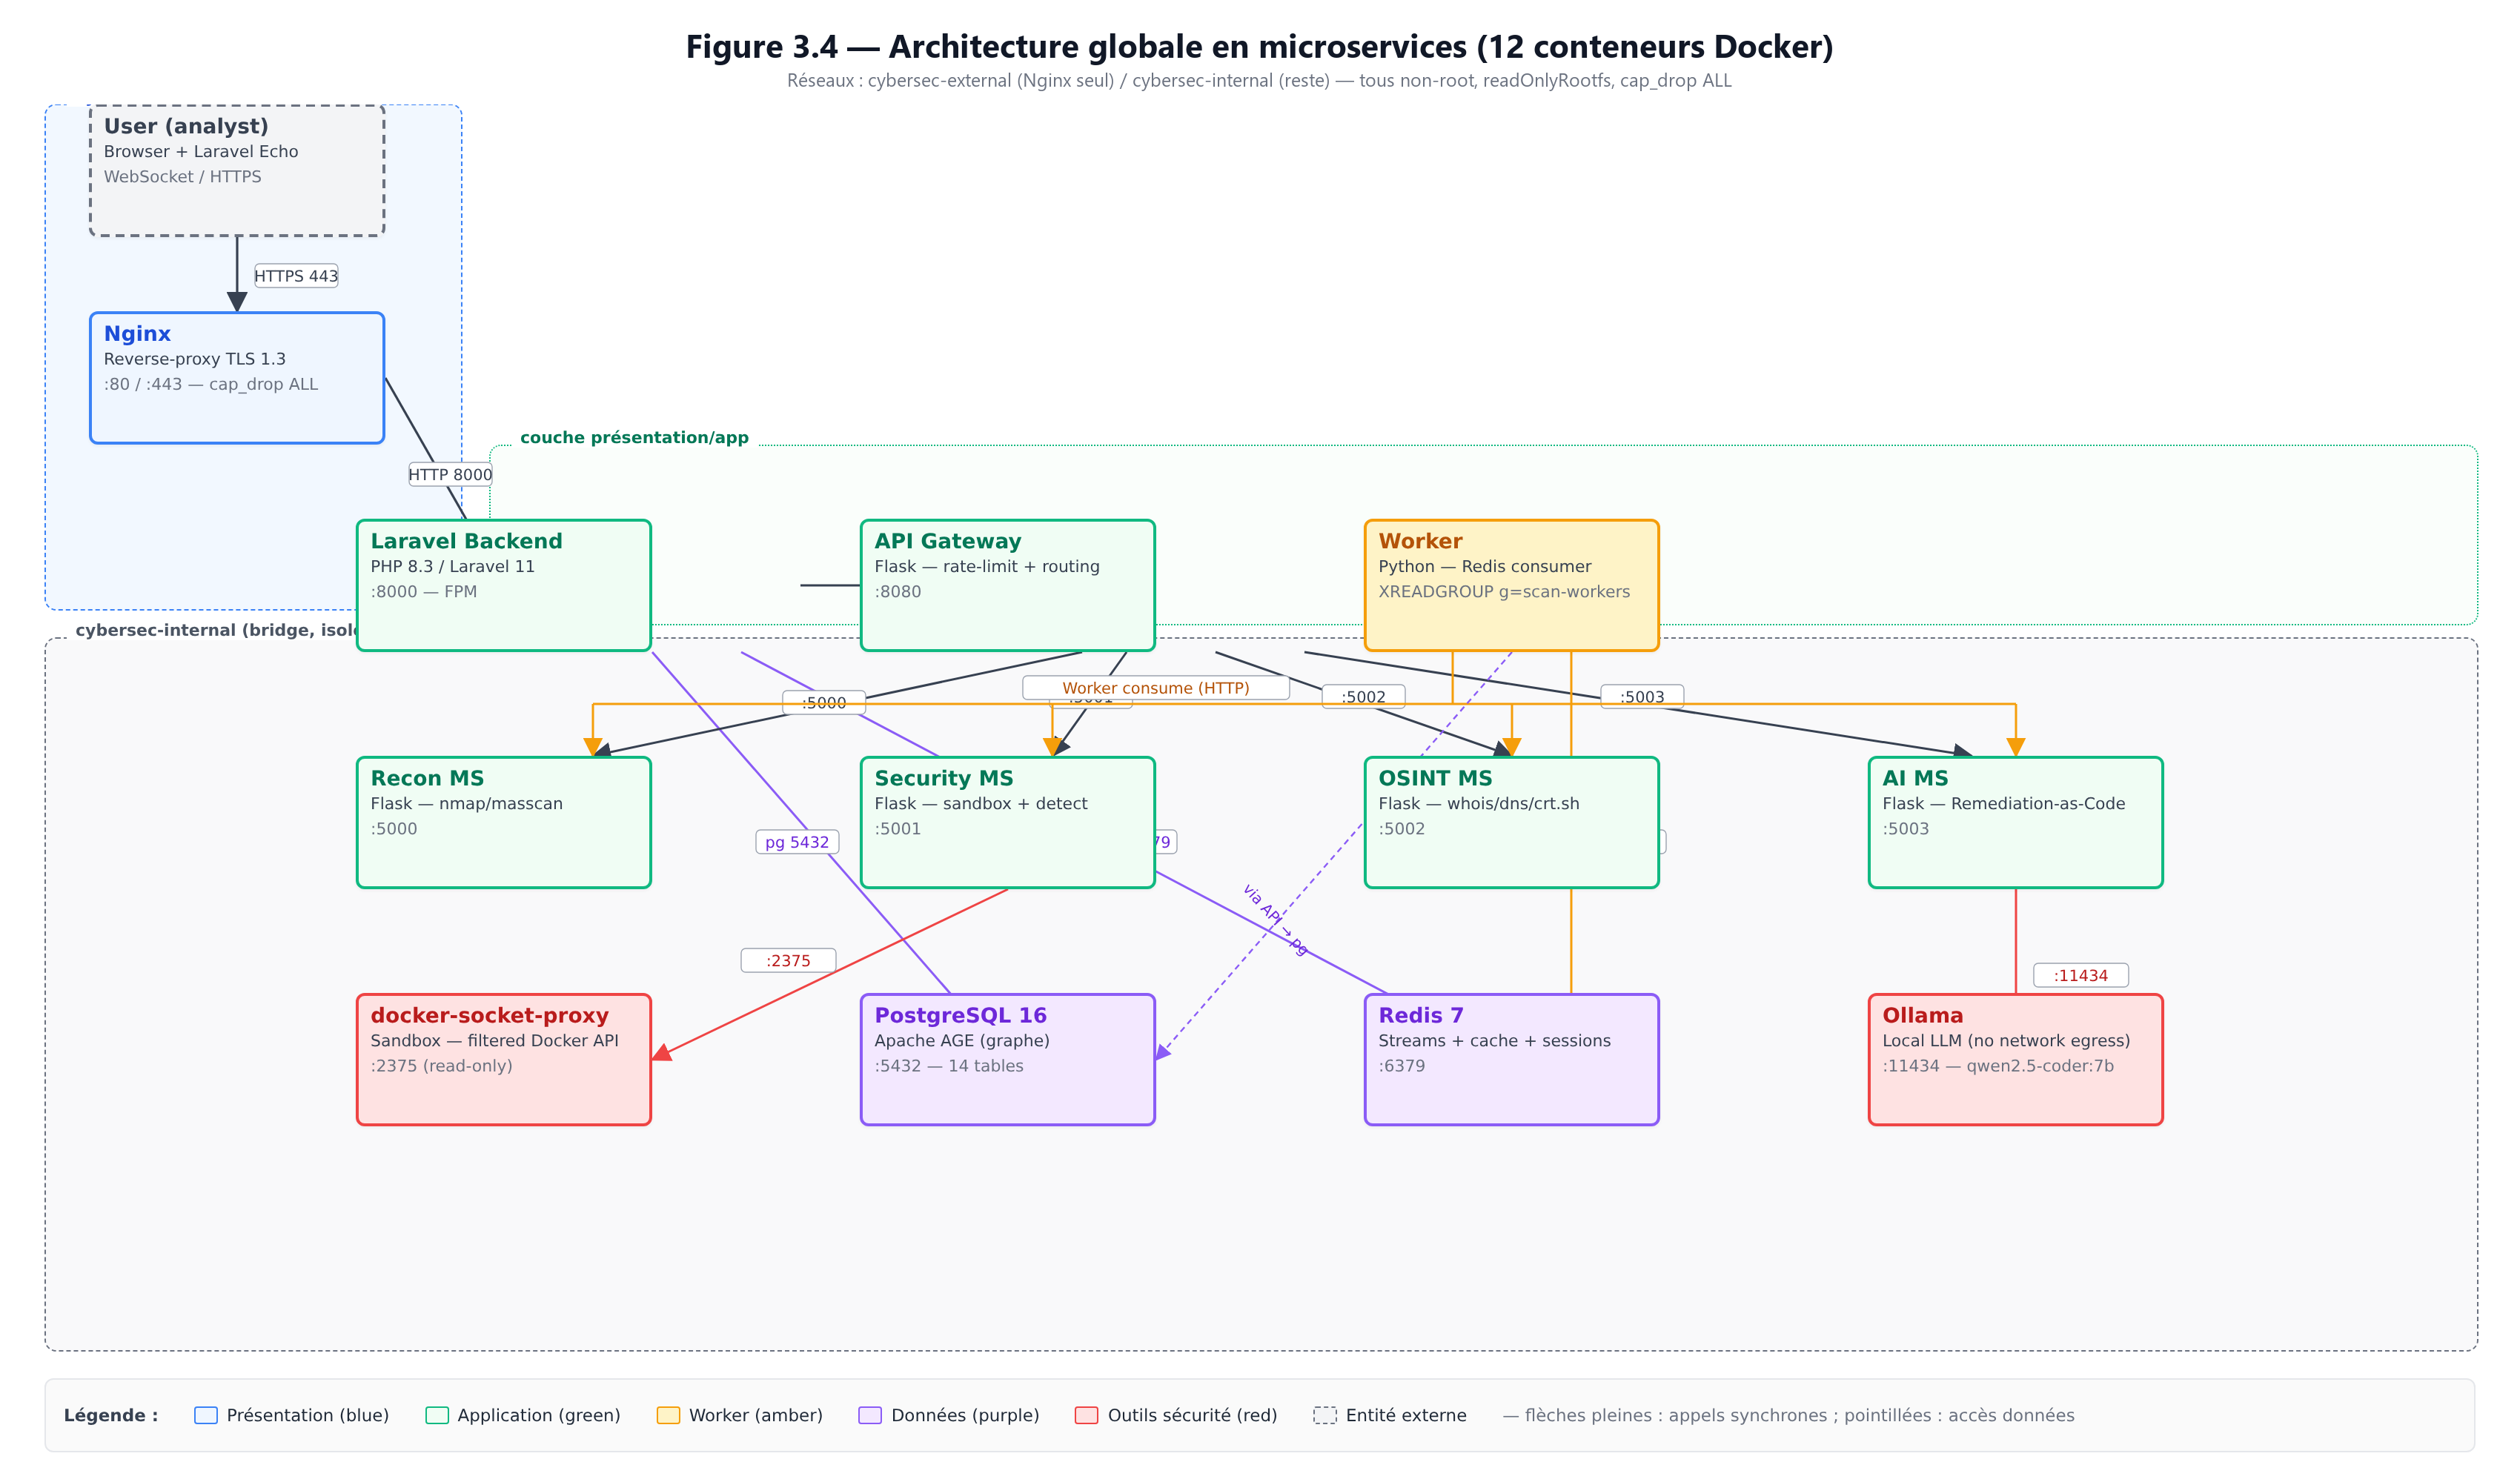
\includegraphics[width=0.92\textwidth]{img/component_diagram.png}
    \caption{Architecture Globale en Microservices -- Vue des 12 Conteneurs Docker et R\'eseaux Segment\'es}
    \label{fig:component_diagram}
\end{figure}

\subsection{Communication Inter-Services}
\par La figure~\ref{fig:ms_comms} pr\'esente la cartographie des flux d'\'echanges internes : requ\^etes REST synchrones, streaming d'\'ev\'enements asynchrones et notifications de mise \`a jour.

\begin{figure}[!htbp]
\centering
\begin{tikzpicture}[
    node distance=8mm and 14mm,
    box/.style={draw, rounded corners=2pt, fill=blue!8, draw=blue!50, thick, minimum width=28mm, minimum height=8mm, align=center, font=\footnotesize},
    sync/.style={-{Stealth[length=2mm]}, thick, draw=green!60!black},
    async/.style={-{Stealth[length=2mm]}, thick, dashed, draw=orange!80!black},
    notify/.style={-{Stealth[length=2mm]}, thick, dotted, draw=red!70!black},
]
\node[box] (browser) {Navigateur (Blade)};
\node[box, right=of browser] (laravel) {Back-end\\Laravel 11};
\node[box, above right=4mm and 16mm of laravel] (recon) {MS Recon\\(Flask :5000)};
\node[box, right=of laravel] (gateway) {Passerelle API\\(Flask :8080)};
\node[box, below right=4mm and 16mm of laravel] (ai) {MS IA\\(Flask :5003)};
\node[box, right=of gateway] (redis) {Redis 7\\Streams};
\node[box, below=of redis] (worker) {Worker\\(Python)};
\node[box, below=of laravel] (pg) {PostgreSQL 16\\+ Apache AGE};
\draw[sync] (browser) -- node[above, font=\tiny]{REST/HTTPS} (laravel);
\draw[sync] (laravel) -- node[above, font=\tiny]{REST} (gateway);
\draw[sync] (gateway) -- (recon);
\draw[sync] (gateway) -- (ai);
\draw[async] (laravel) -- node[right, font=\tiny]{XADD} (redis);
\draw[async] (redis) -- node[right, font=\tiny]{XREADGROUP} (worker);
\draw[async] (worker) -- node[below, font=\tiny]{r\'esultats} (pg);
\draw[notify] (pg) -- node[left, font=\tiny]{NOTIFY} (laravel);
\draw[notify] (recon) -- node[below, font=\tiny]{insert} (pg);
\end{tikzpicture}
\caption{Flux de Communication du Traitement Asynchrone d'un Scan -- REST Synchrone, Redis Streams et PostgreSQL NOTIFY}
\label{fig:ms_comms}
\end{figure}

\subsection{Communication Synchrone REST vs Asynchrone par \'Ev\'enements}
\par La plateforme combine deux paradigmes d'\'echange compl\'ementaires :
\begin{itemize}
    \item \textbf{Communication synchrone REST (HTTP/JSON) :} R\'eserv\'ee aux requ\^etes imm\'ediates (interrogation du tableau de bord, requ\^etes OSINT rapides, inf\'erence de dialogue IA).
    \item \textbf{Communication asynchrone (Redis Streams) :} Utilis\'ee pour l'ex\'ecution des scanners lourds. Le back-end publie un message (\texttt{XADD}), imm\'ediatement acquitt\'e pour l'utilisateur, tandis que le worker d\'epile le travail en arri\`ere-plan sans bloquer l'IHM.
\end{itemize}

\section{Conception des Donn\'ees et Dynamique du Syst\`eme}
\subsection{Mod\`ele Entit\'e-Association (ERD)}
\par La base de donn\'ees structure 14 tables relationnelles li\'ees par des contraintes d'int\'egrit\'e r\'ef\'erentielle strictes et enrichies de colonnes \texttt{JSONB} index\'ees par index GIN.

\begin{figure}[!htbp]
    \centering
    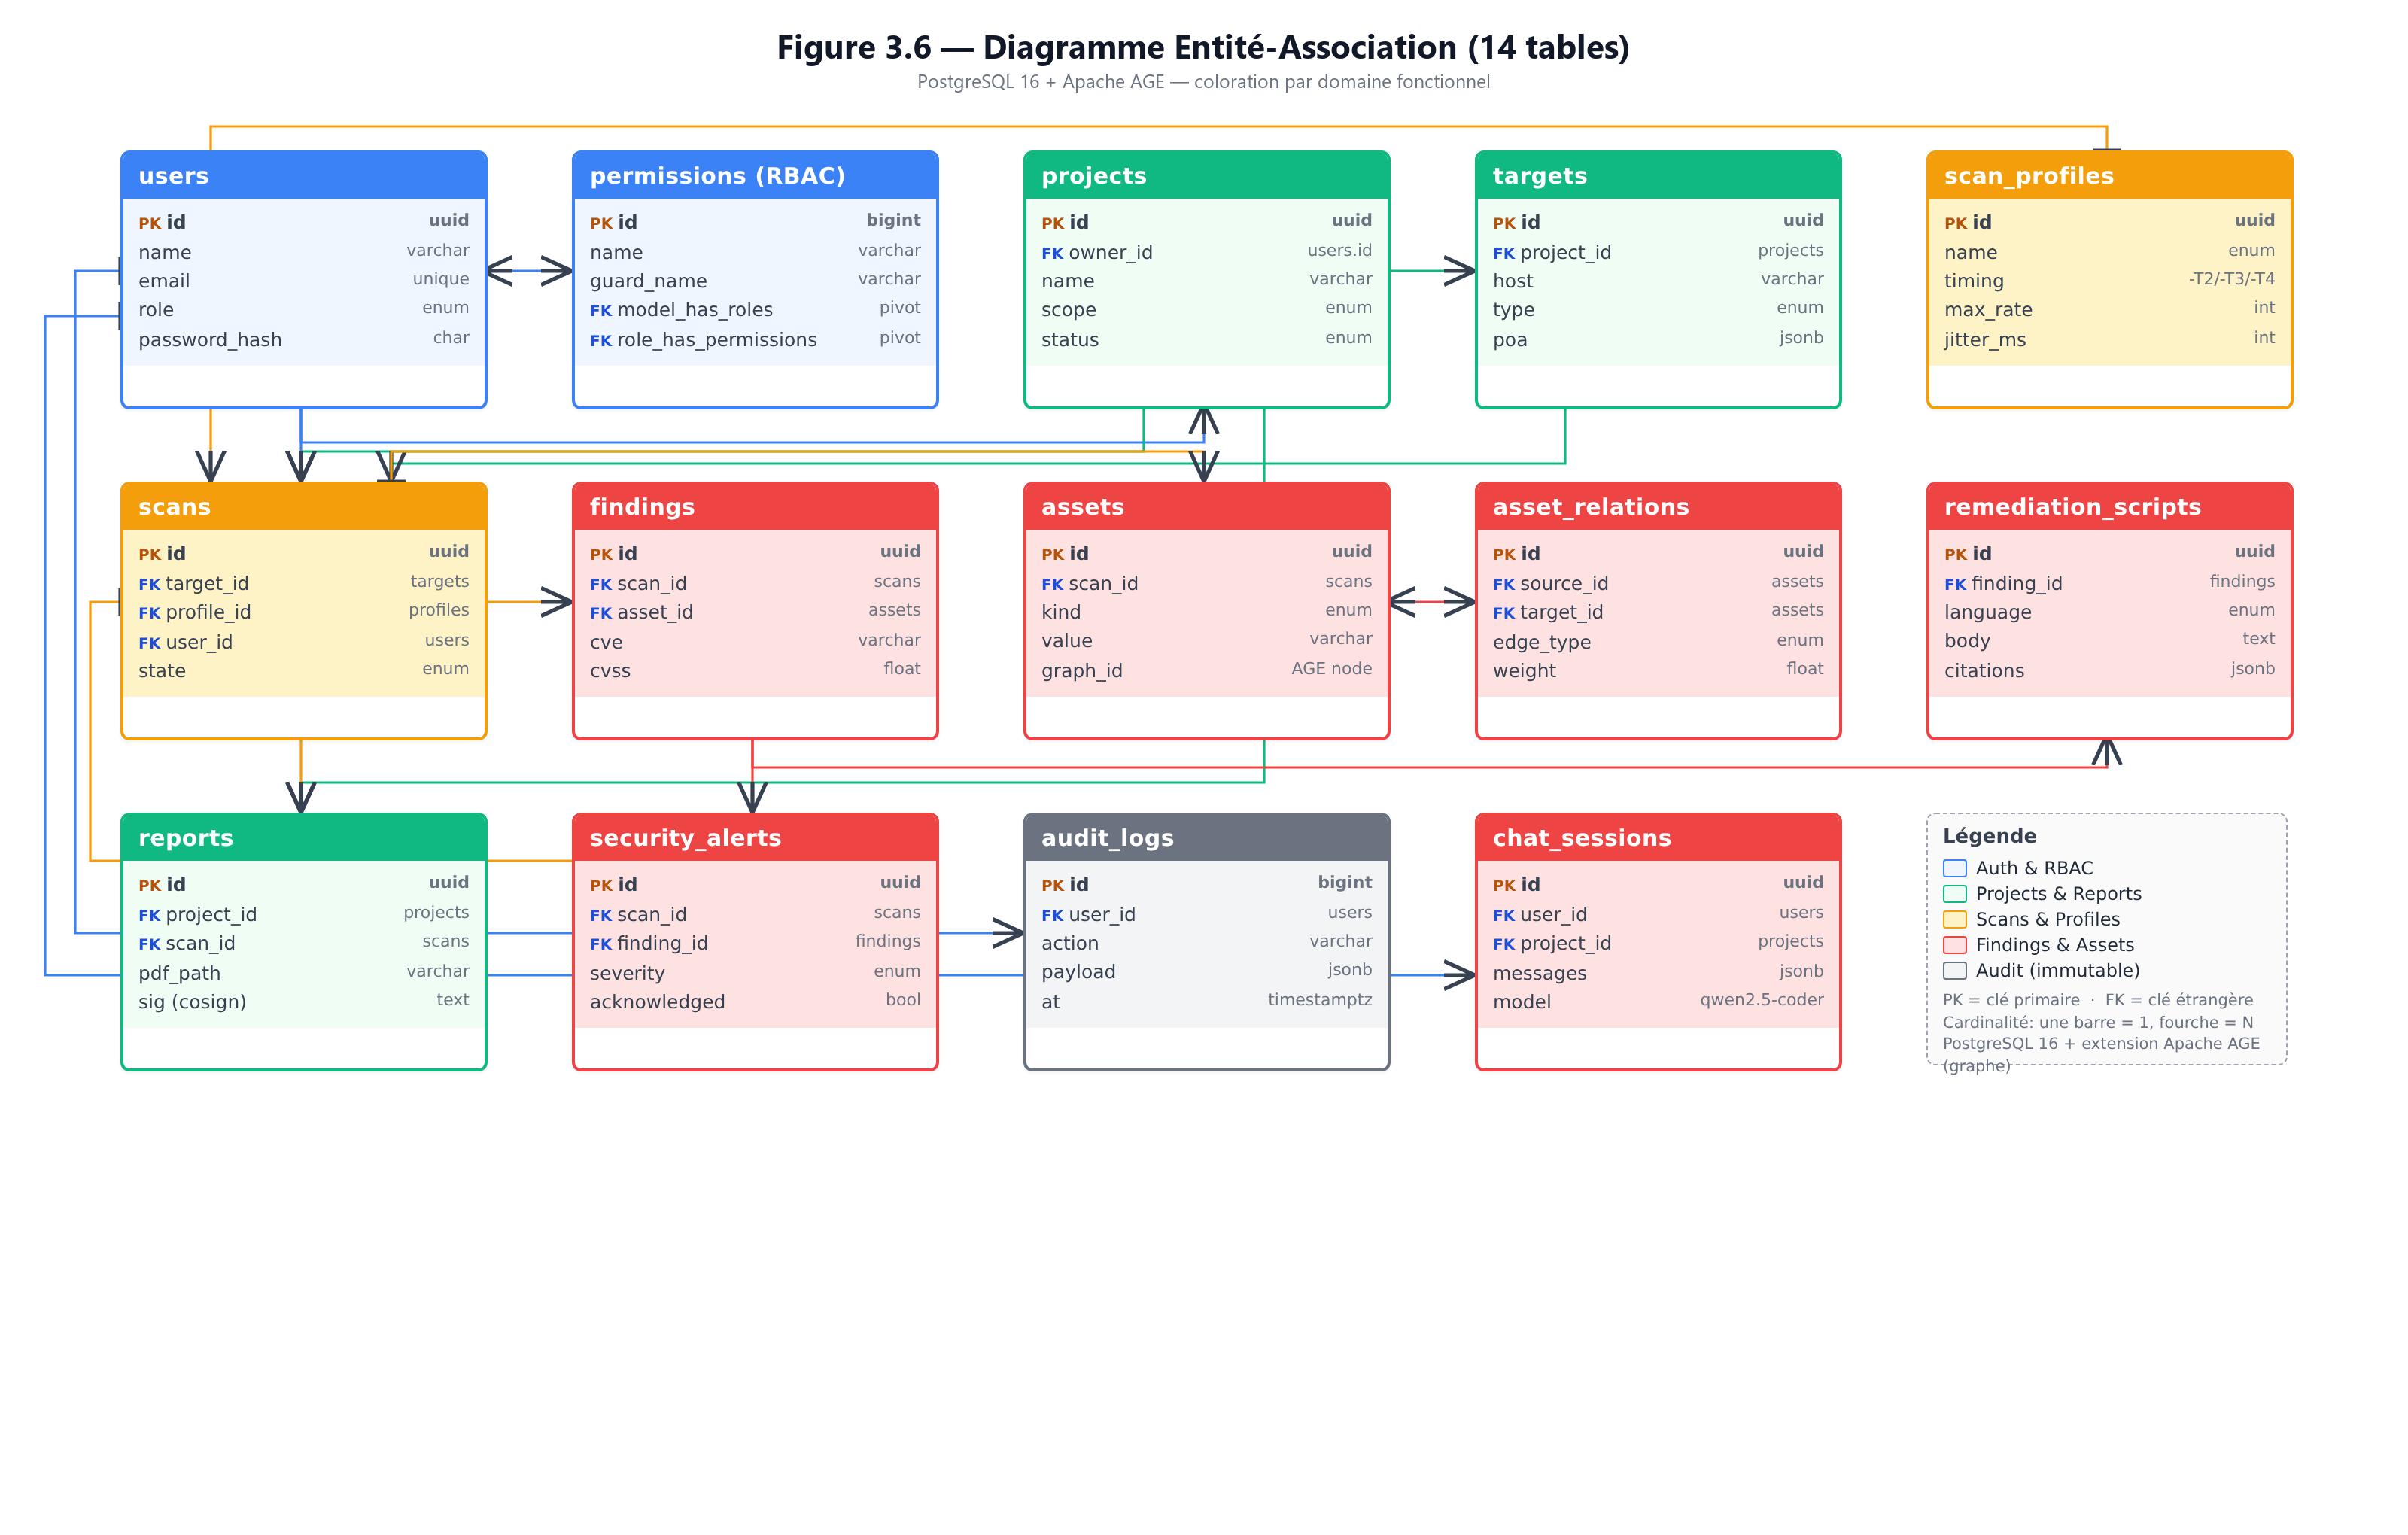
\includegraphics[width=0.92\textwidth]{img/erd.png}
    \caption{Mod\`ele Entit\'e-Association (ERD) -- Les 14 Tables de la Plateforme}
    \label{fig:erd_diagram}
\end{figure}

\subsection{Diagramme de Classes du Mod\`ele de Donn\'ees}
\par Tandis que le Mod\`ele Entit\'e-Association (ERD) formalise la structure relationnelle et physique de la base de donn\'ees, le diagramme de classes repr\'esente la structure logique des principales entit\'es m\'etier et leurs relations au sein du framework applicatif. La structure objet et les relations cardinales entre les entit\'es sont illustr\'ees dans la figure~\ref{fig:class_diagram}.

\begin{figure}[!htbp]
    \centering
    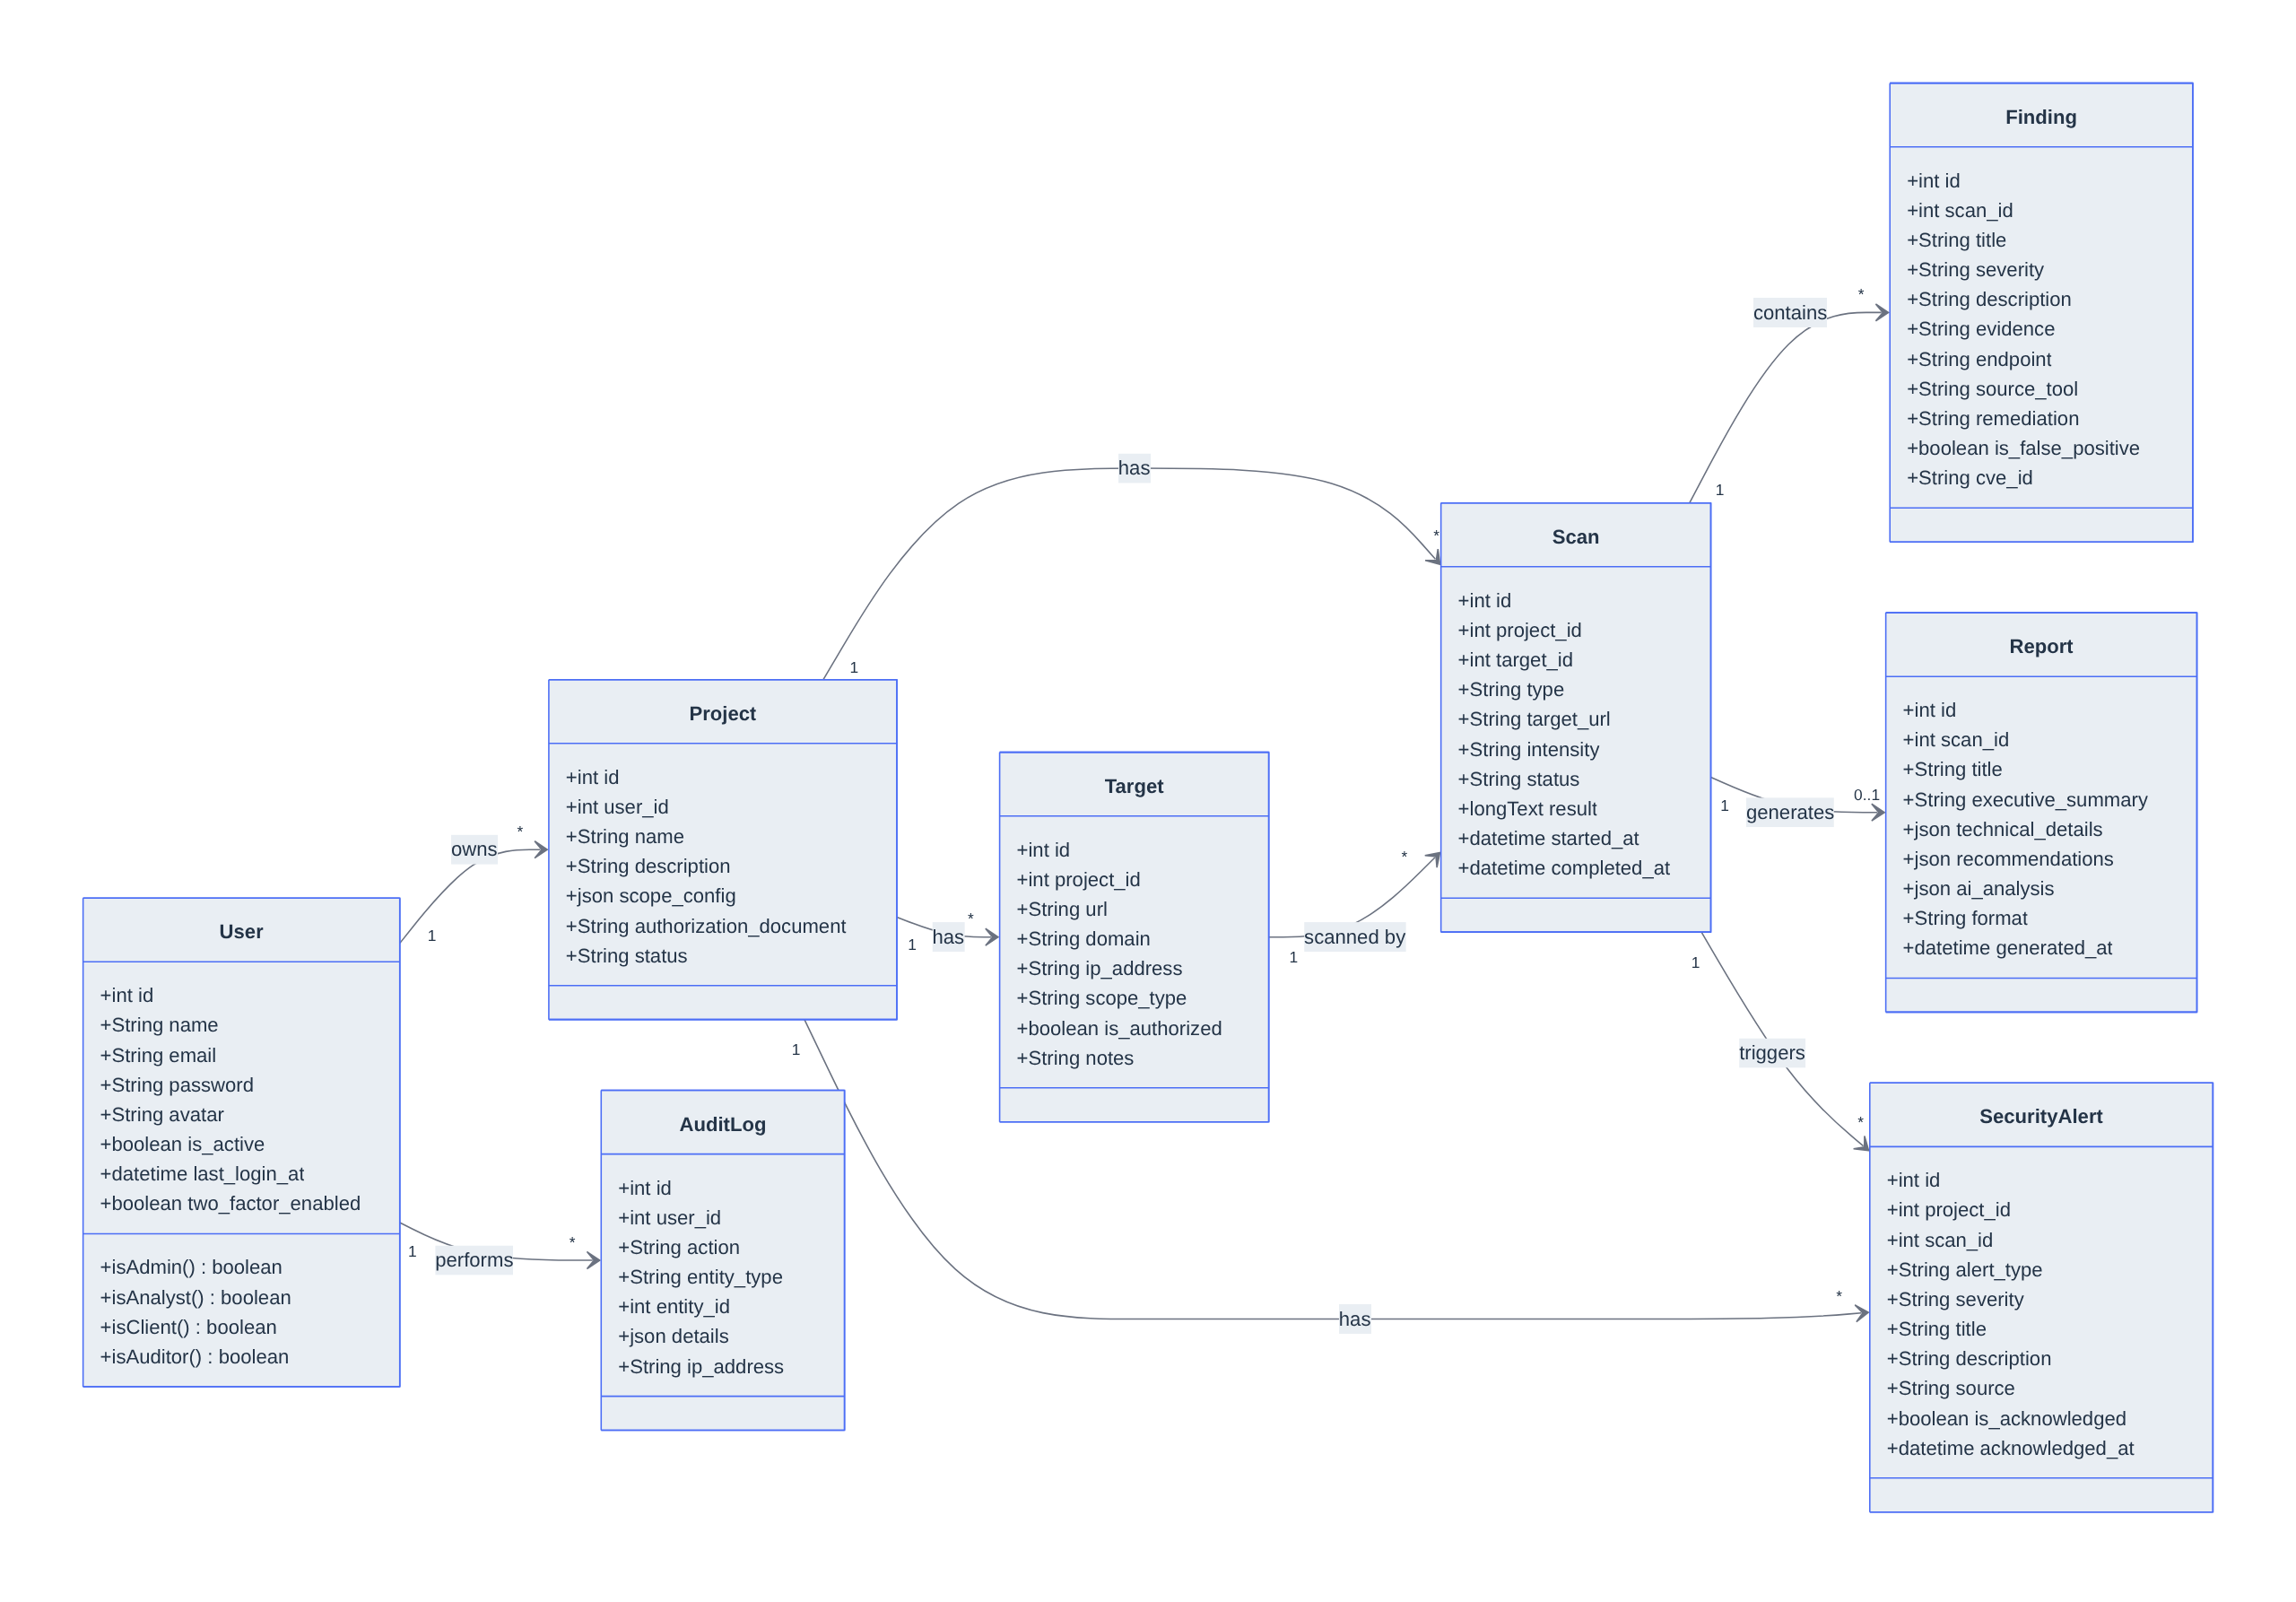
\includegraphics[width=0.90\textwidth]{img/class_diagram.png}
    \caption{Diagramme de Classes -- Entit\'es M\'etier et Relations du Mod\`ele}
    \label{fig:class_diagram}
\end{figure}

\subsection{Mod\`ele du Graphe de Connaissances et Projection Apache AGE}
\par Les relations de s\'ecurit\'e sont mod\'elis\'ees sous forme de n\oe uds (\textit{Target}, \textit{Asset}, \textit{Port}, \textit{Service}, \textit{Vulnerability}) et d'ar\^etes typ\'ees (\textit{RESOLVES\_TO}, \textit{HOSTS}, \textit{RUNS}, \textit{HAS\_VULN}, \textit{IMPACTS}). Cette mod\'elisation permet de calculer le rayon d'impact (\textit{blast radius}) par parcours de graphe en largeur (BFS) impl\'ement\'e sous NetworkX.

\subsection{Diagramme de S\'equence du D\'eroulement d'un Scan}
\par La figure~\ref{fig:sequence_scan} mod\'elise la s\'equence d'ex\'ecution compl\`ete d'un audit de reconnaissance, de la soumission initiale jusqu'\`a la persistance des constats et \`a l'analyse IA.

\begin{figure}[!htbp]
    \centering
    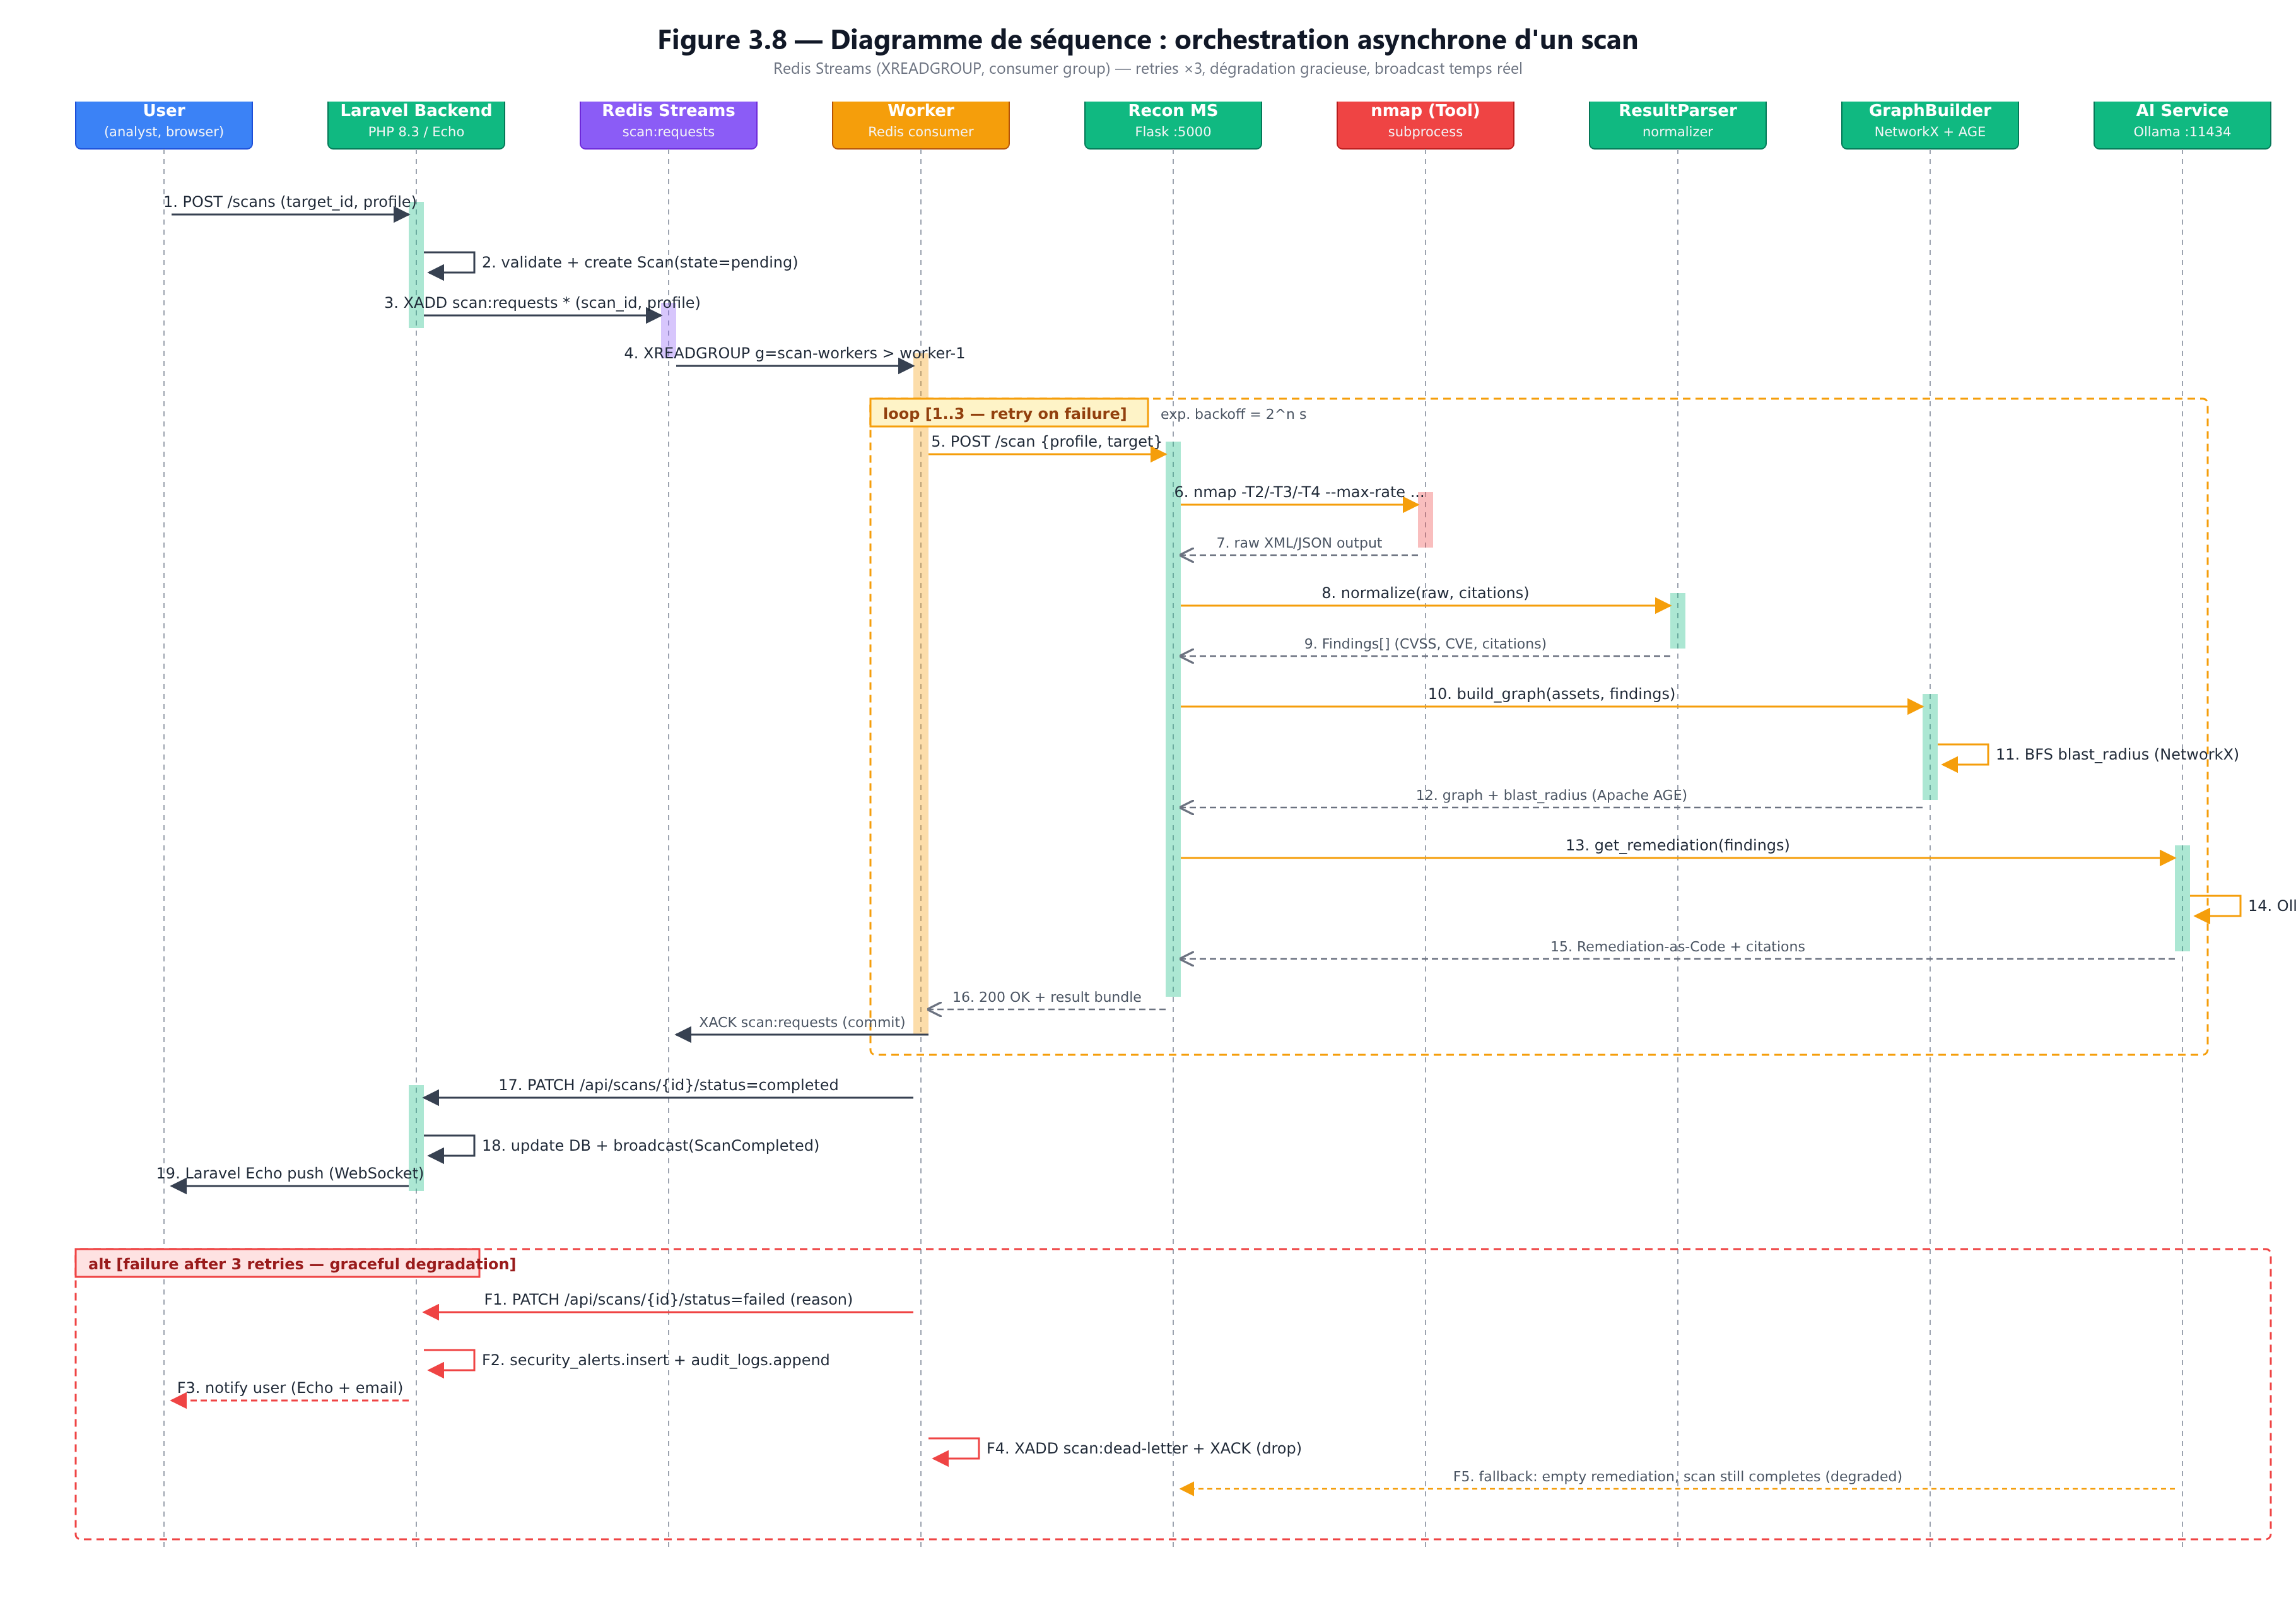
\includegraphics[width=0.92\textwidth]{img/sequence_scan.png}
    \caption{Diagramme de S\'equence -- Orchestration Asynchrone d'un Scan}
    \label{fig:sequence_scan}
\end{figure}

\subsection{Machine \`a \'Etats d'un Scan}
\par Le cycle de vie d'une t\^ache de scan est r\'egi par une machine \`a \'etats finis d\'eterministe comprenant les \'etats \texttt{Pending}, \texttt{Queued}, \texttt{Running}, \texttt{Completed}, \texttt{Failed} et \texttt{Cancelled}.

\begin{figure}[!htbp]
    \centering
    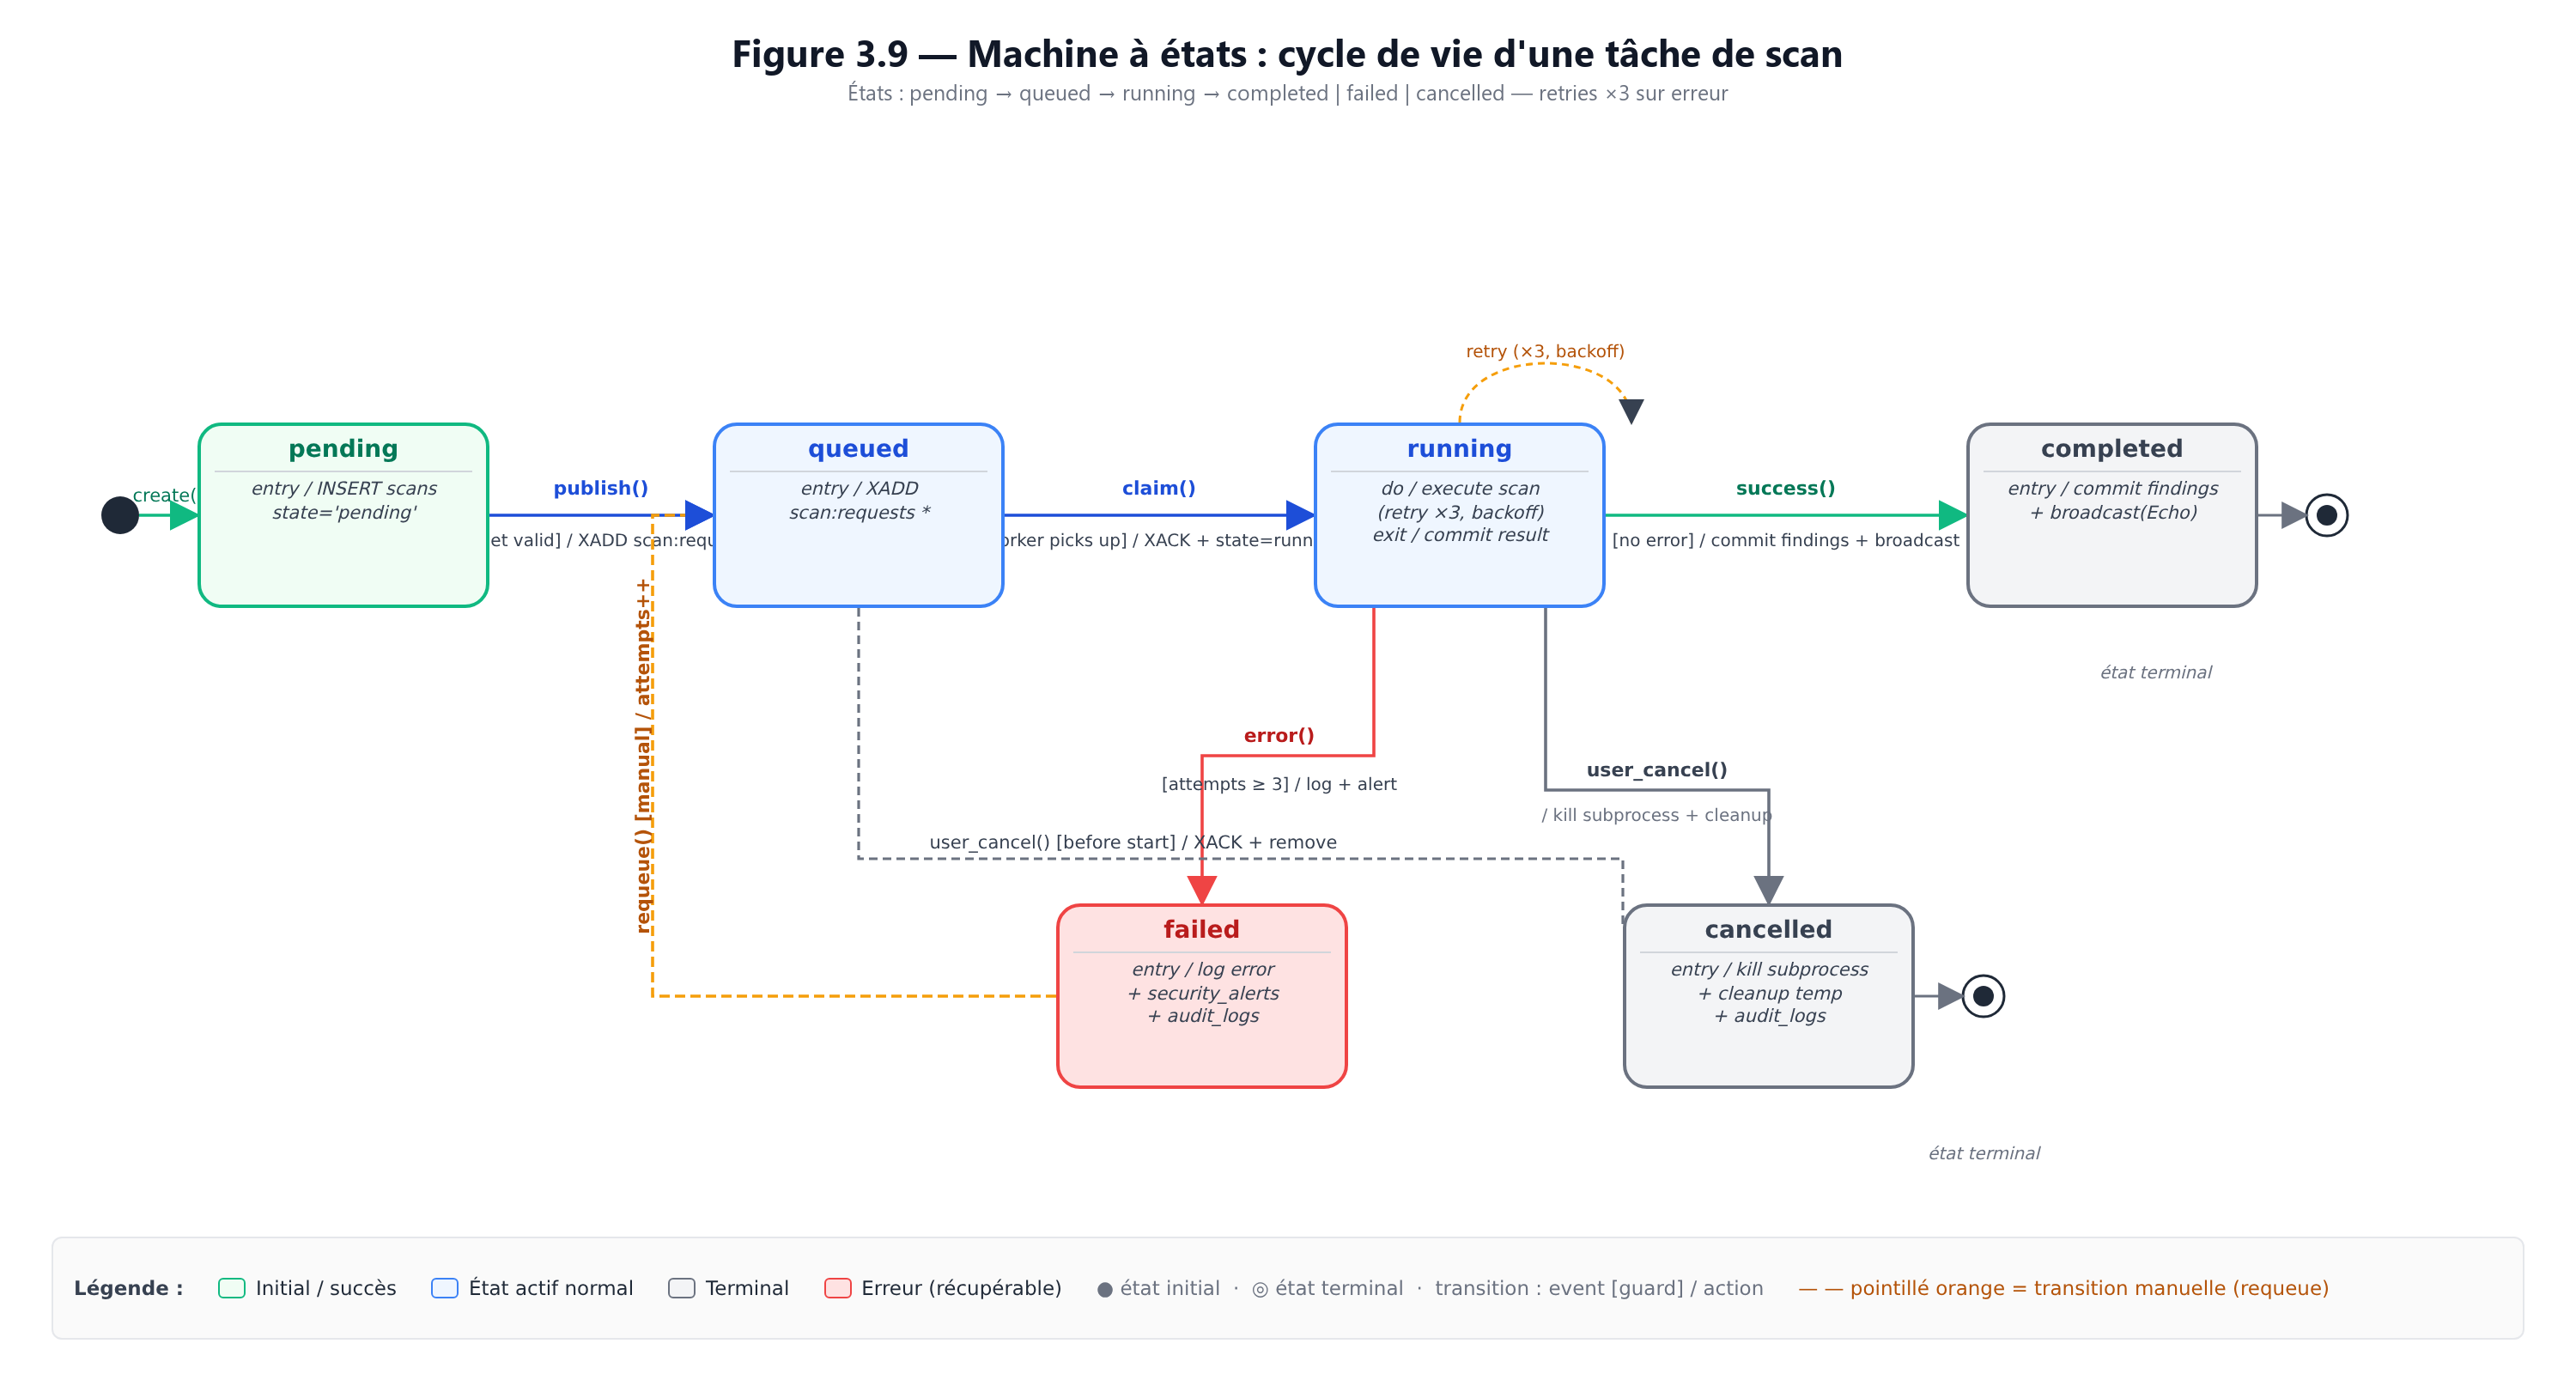
\includegraphics[width=0.85\textwidth]{img/state_machine.png}
    \caption{Machine \`a \'Etats -- Cycle de Vie d'une T\^ache de Scan}
    \label{fig:state_machine}
\end{figure}

\subsection{Diagramme de Flux de Donn\'ees (DFD)}
\par Le cheminement et les transformations successives des donn\'ees sont synth\'etis\'es dans le diagramme de flux de la figure~\ref{fig:data_flow}.

\begin{figure}[!htbp]
    \centering
    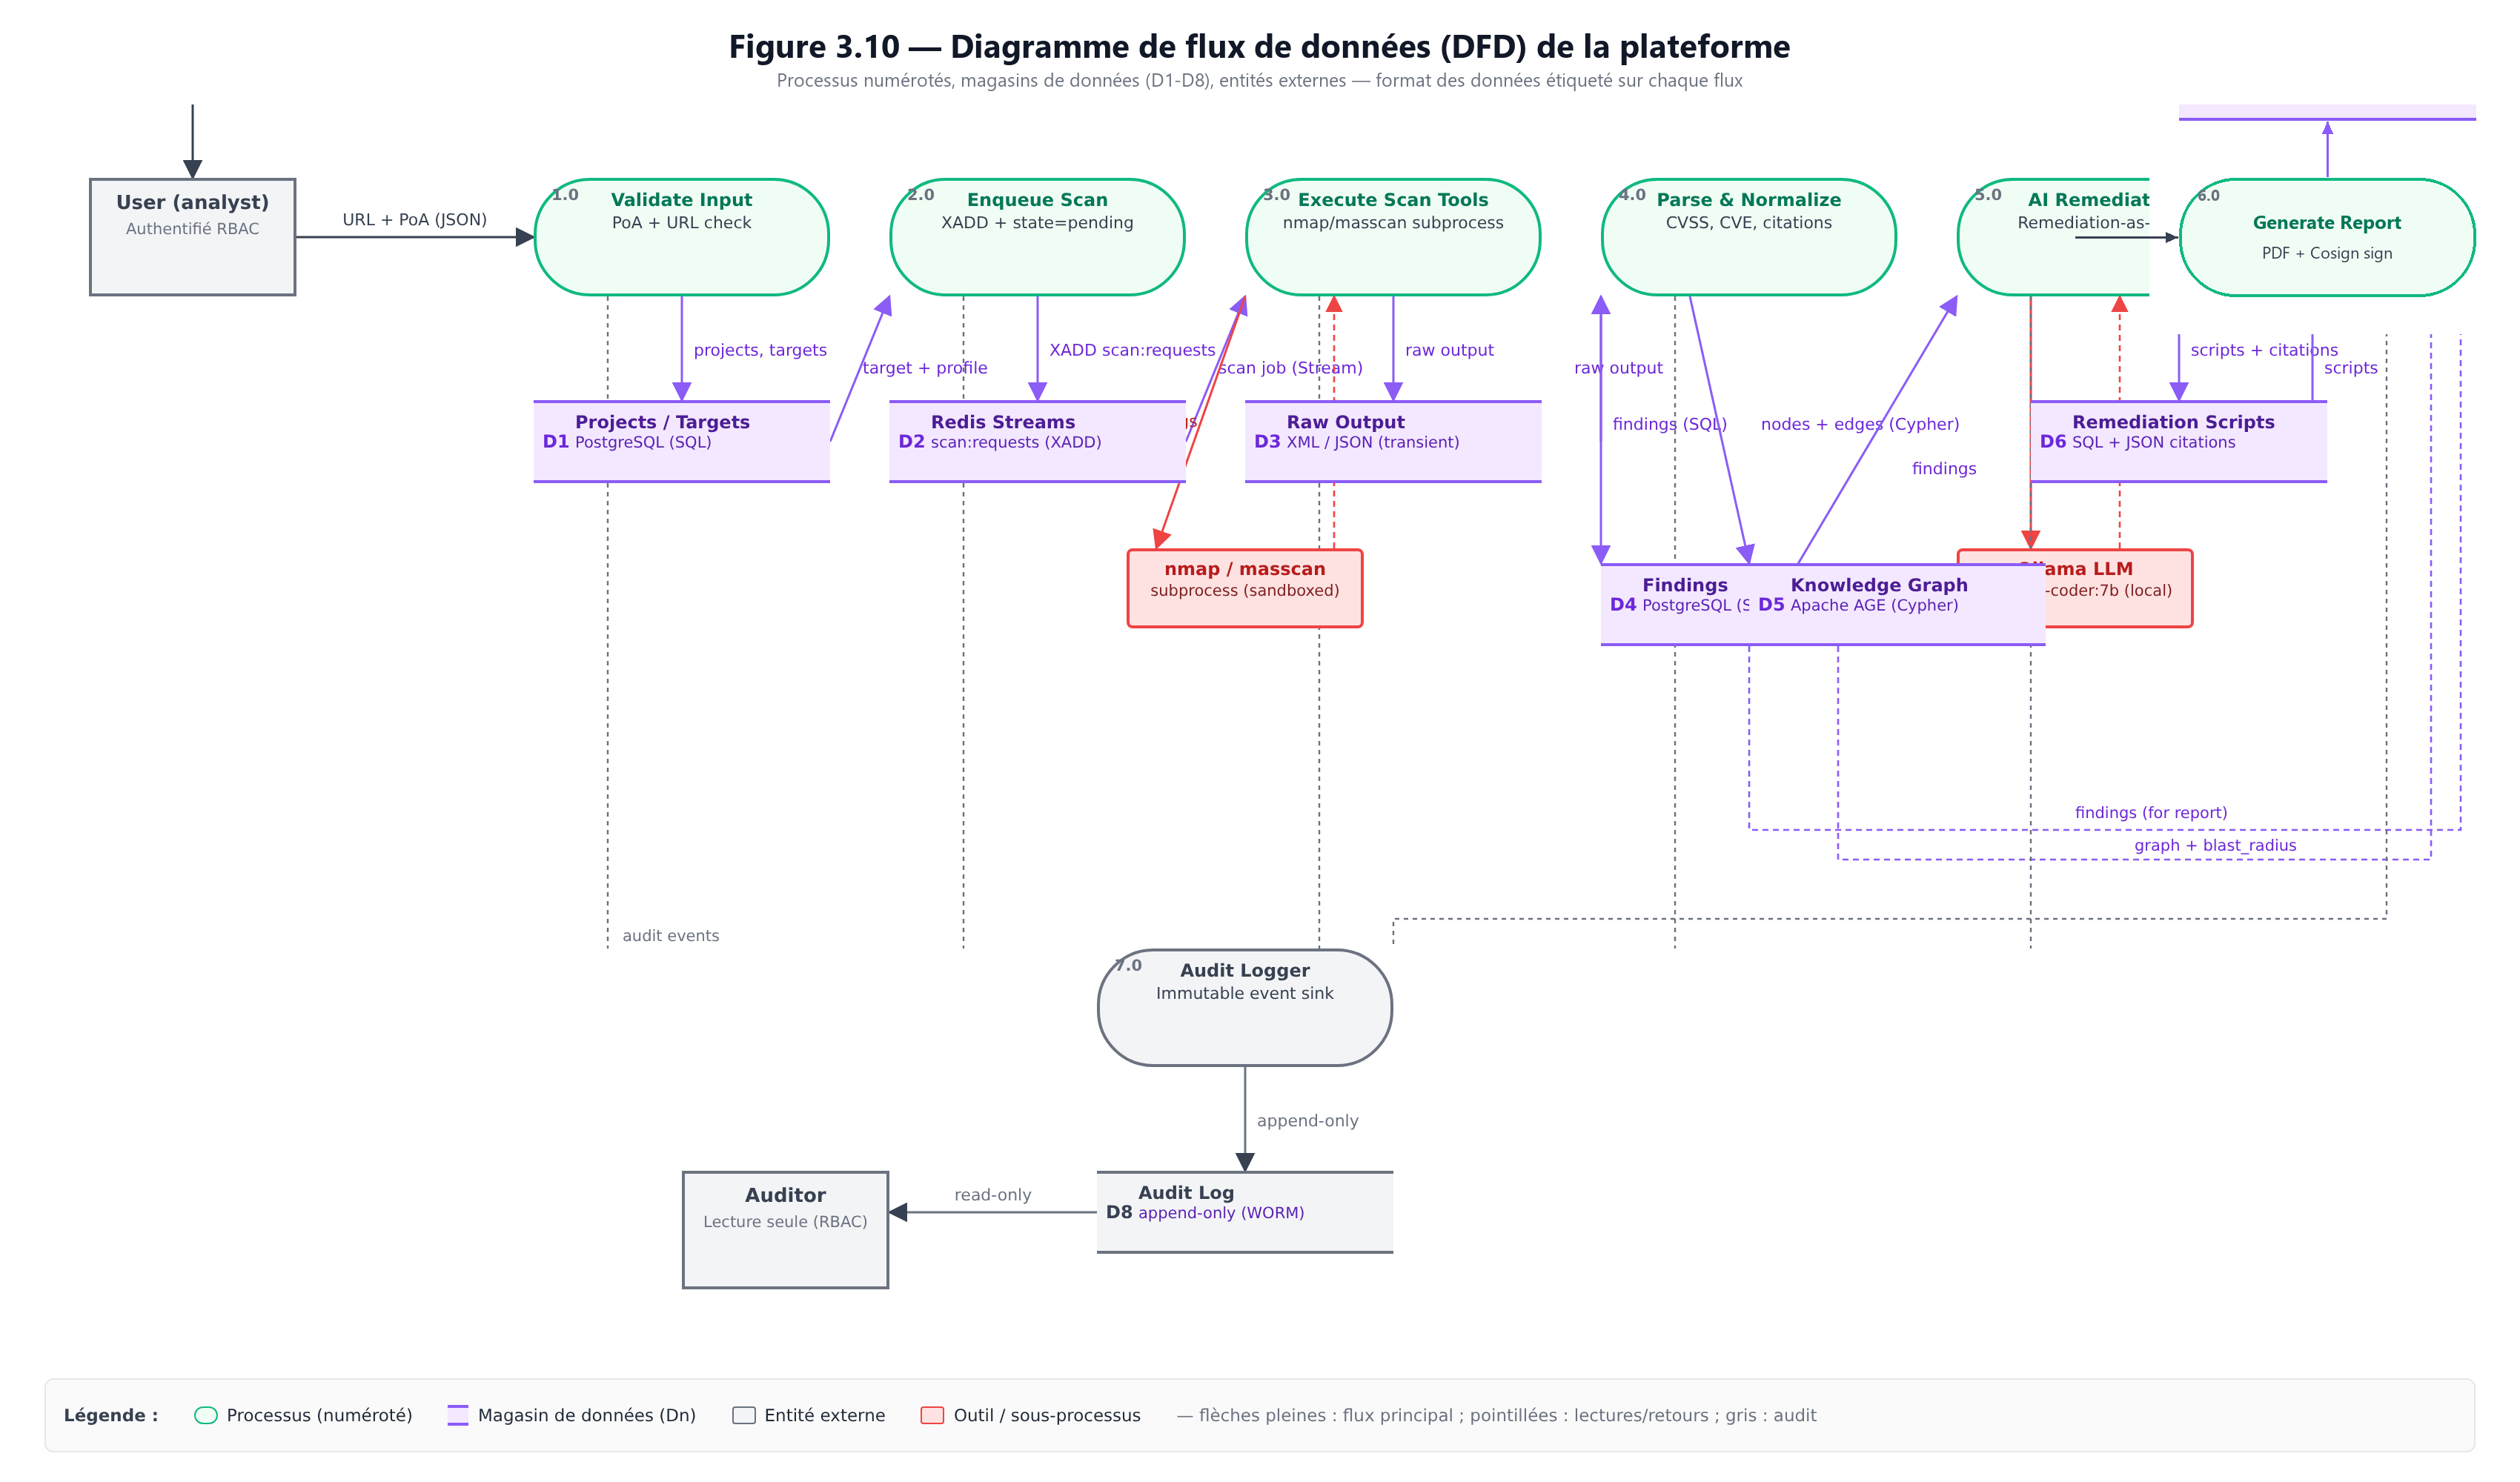
\includegraphics[width=0.92\textwidth]{img/data_flow.png}
    \caption{Diagramme de Flux de Donn\'ees (DFD) -- Processus d'Audit, Graphe de Connaissances et Reporting}
    \label{fig:data_flow}
\end{figure}

\section{Architecture de S\'ecurit\'e Multicouche}
\par Afin de prot\'eger la plateforme elle-m\^eme contre toute compromission, nous appliquons une d\'efense en profondeur (\textit{Defense-in-Depth}) sur six niveaux :
\begin{enumerate}
    \item \textbf{S\'ecurit\'e R\'eseau et Segmentation :} R\'epartition en deux r\'eseaux bridges Docker isol\'es : \texttt{cybersec-external} (exposant uniquement Nginx sur les ports 80/443) et \texttt{cybersec-internal} (inaccessible depuis l'ext\'erieur, r\'eserv\'e aux communications inter-microservices et bases de donn\'ees).
    \item \textbf{S\'ecurit\'e des Conteneurs :} Ex\'ecution de tous les microservices sous utilisateur non-root (\texttt{UID 1001:1001}), syst\`eme de fichiers racine mont\'e en lecture seule (\texttt{read\_only: true}), et suppression de toutes les capabilit\'es Linux superflues (\texttt{cap\_drop: [ALL]}).
    \item \textbf{S\'ecurit\'e Applicative :} Authentification par jetons s\'ecuris\'es Laravel Sanctum, protection native contre les failles CSRF, XSS et injections SQL, limitation de d\'ebit (\textit{rate limiting}) et validation stricte des param\`etres HTTP.
    \item \textbf{S\'ecurit\'e des Donn\'ees :} Chiffrement des mots de passe en \texttt{bcrypt}, chiffrement des cl\'es d'API sensibles, journalisation d'audit immuable et politique de purge automatique RGPD.
    \item \textbf{Mod\`ele de Contr\^ole d'Acc\`es RBAC :} Attribution granulaire des permissions selon quatre r\^oles stricts (Admin, Analyste, Client, Auditeur).
    \item \textbf{Isolation du Bac \`a Sable (Sandbox) :} Les conteneurs de test vuln\'erables (DVWA, SQLi-Labs) sont pilot\'es \`a travers \texttt{docker-socket-proxy} qui filtre et d\'esactive formellement les commandes Docker dangereuses (suppression d'images, acc\`es aux volumes de production).
\end{enumerate}

\section{Mod\'elisation Formelle des Menaces (Threat Modeling STRIDE)}
\subsection{M\'ethodologie et Fronti\`eres de Confiance}
\par Une plateforme de reconnaissance offensive concentre par nature des outils puissants et des informations critiques de vuln\'erabilit\'e. Elle constitue par cons\'equent une cible de choix pour des attaquants. Afin d'\'evaluer m\'ethodiquement les risques pesant sur le syst\`eme, nous avons appliqu\'e la m\'ethodologie de mod\'elisation des menaces \textbf{STRIDE} d\'evelopp\'ee par Microsoft.
\par La figure~\ref{fig:trust_boundaries} illustre la cartographie des fronti\`eres de confiance (\textit{Trust Boundaries}) et l'exposition de la surface d'attaque interne de la plateforme.

\begin{figure}[!htbp]
\centering
\begin{tikzpicture}[
    node distance=6mm and 10mm,
    zone/.style={draw, dashed, rounded corners=4pt, inner sep=6pt, font=\scriptsize\bfseries},
    box/.style={draw, rounded corners=2pt, fill=blue!8, draw=blue!50, thick, minimum width=24mm, minimum height=8mm, align=center, font=\footnotesize},
    ext/.style={draw, rounded corners=2pt, fill=gray!15, draw=gray!60, thick, minimum width=22mm, minimum height=8mm, align=center, font=\footnotesize},
    tb/.style={draw=red!70, thick, dashed},
    arrow/.style={-{Stealth[length=2mm]}, thick, draw=gray!80},
]
\node[ext] (internet) {Internet Public\\(Attaquants / Clients)};
\node[box, right=14mm of internet] (nginx) {Nginx 1.27\\(DMZ / TLS 1.3)};
\node[box, right=14mm of nginx] (laravel) {Back-end\\Laravel 11};
\node[box, above right=2mm and 10mm of laravel] (recon) {MS Recon\\(Flask)};
\node[box, right=10mm of laravel] (redis) {Redis 7 / PG 16\\(AGE Graph)};
\node[box, below right=2mm and 10mm of laravel] (ai) {MS IA / Ollama\\(qwen2.5-coder)};
\node[box, right=10mm of recon] (sandbox) {Sandbox\\(DVWA / SQLi)};

\draw[arrow] (internet) -- node[above, font=\tiny]{HTTPS (443)} (nginx);
\draw[arrow] (nginx) -- node[above, font=\tiny]{FastCGI / HTTP} (laravel);
\draw[arrow] (laravel) -- (recon);
\draw[arrow] (laravel) -- (redis);
\draw[arrow] (laravel) -- (ai);
\draw[arrow] (recon) -- (sandbox);

% Trust Boundary lines
\draw[tb] (2.2, 2.2) -- (2.2, -2.2) node[pos=0.05, right, font=\tiny\color{red!70}]{TB1: Fronti\`ere Externe};
\draw[tb] (5.8, 2.2) -- (5.8, -2.2) node[pos=0.05, right, font=\tiny\color{red!70}]{TB2: Fronti\`ere Applicative};
\draw[tb] (10.6, 2.2) -- (10.6, -2.2) node[pos=0.05, right, font=\tiny\color{red!70}]{TB3: Fronti\`ere Sandbox};
\end{tikzpicture}
\caption{Cartographie de la Surface d'Attaque et Fronti\`eres de Confiance (Trust Boundaries)}
\label{fig:trust_boundaries}
\end{figure}

\subsection{Matrice des Menaces STRIDE et Contre-Mesures Appliqu\'ees}
\par Le tableau~\ref{tab:stride_matrix} d\'etaille l'analyse syst\'ematique des six cat\'egories de menaces STRIDE sur chaque composant cl\'e de la plateforme, le niveau de risque associ\'e et les contre-mesures architecturales impl\'ement\'ees.

\begin{table}[H]
\centering
\caption{Matrice d'Analyse des Menaces STRIDE et Contre-Mesures Architecturales}
\label{tab:stride_matrix}
\resizebox{\textwidth}{!}{%
\begin{tabular}{|L|L|C|L|}
\hline
\textbf{Composant Cibl\'e} & \textbf{Menace STRIDE Identifi\'ee} & \textbf{Niveau de Risque} & \textbf{Contre-Mesures et Att\'enuations Impl\'ement\'ees} \\
\hline
Passerelle Nginx & \textbf{S}poofing / Usurpation d'identit\'e & \'Elev\'e & Terminaison TLS 1.3 avec HSTS, validation stricte des certificats Let's Encrypt \\
\hline
Back-end Laravel & \textbf{T}ampering / Alt\'eration des donn\'ees & \'Elev\'e & Requ\^etes pr\'epar\'ees Eloquent (anti-SQLi), protection CSRF native, assainissement HTML \\
\hline
Syst\`eme de Journalisation & \textbf{R}epudiation / R\'epudiation d'actions & Moyen & Piste d'audit immuable (\textit{Audit Log}) horodat\'ee avec tra\c{c}abilit\'e \texttt{X-Correlation-ID} \\
\hline
Base PostgreSQL / AGE & \textbf{I}nformation Disclosure / Fuite d'infos & Critique & R\'eseau priv\'e \texttt{cybersec-internal} non expos\'e, chiffrement des cl\'es d'API au repos \\
\hline
Files Redis Streams & \textbf{D}enial of Service / D\'eni de service & \'Elev\'e & Quotas stricts de scans simultan\'es par utilisateur, limitation de d\'ebit (\textit{rate limiting}) \\
\hline
Microservice Sandbox & \textbf{E}levation of Privilege / \'Evasion Docker & Critique & Isolation via \texttt{docker-socket-proxy}, conteneurs non-root (UID 1001), \texttt{cap\_drop: ALL} \\
\hline
Microservice IA (Ollama) & \textbf{T}ampering / Injection de Prompts & \'Elev\'e & \textit{System prompt} fig\'e, validation de sch\'ema JSON strict et v\'erification des citations de logs \\
\hline
Moteur de Scanners & Ex\'ecution sur cible non autoris\'ee & Critique & Barri\`ere logicielle bloquante : v\'erification obligatoire du mandat d'autorisation (PoA) \\
\hline
\end{tabular}}%
\end{table}

\section{Architecture DevSecOps D\'etaill\'ee}
\subsection{Pipeline CI/CD sous GitHub Actions}
\par La s\'ecurit\'e de la cha\^ine logicielle est enti\`erement automatis\'ee au sein du d\'ep\^ot de code via le workflow GitHub Actions d\'eclar\'e dans \texttt{.github/workflows/devsecops.yml}. Chaque commit et requ\^ete de tirage (\textit{pull request}) d\'eclenche l'ex\'ecution de huit \'etapes successives bloquantes.

\begin{figure}[!htbp]
\centering
\begin{tikzpicture}[
    node distance=4mm and 6mm,
    stage/.style={draw, rounded corners=3pt, fill=violet!10, draw=violet!60, thick, minimum width=24mm, minimum height=10mm, align=center, font=\footnotesize},
    arrow/.style={-{Stealth[length=2.2mm]}, thick, draw=violet!70},
]
\node[stage] (s1) {1.~Commit\\Source};
\node[stage, right=of s1] (s2) {2.~SAST\\(psalm, bandit)};
\node[stage, right=of s2] (s3) {3.~SCA\\(trivy fs)};
\node[stage, right=of s3] (s4) {4.~SBOM\\(syft)};
\node[stage, below=6mm of s4] (s5) {5.~Build\\Docker};
\node[stage, left=of s5] (s6) {6.~Image Scan\\(trivy image)};
\node[stage, left=of s6] (s7) {7.~Signature\\(cosign)};
\node[stage, left=of s7] (s8) {8.~D\'eploiement\\Production};

\draw[arrow] (s1) -- (s2);
\draw[arrow] (s2) -- (s3);
\draw[arrow] (s3) -- (s4);
\draw[arrow] (s4) -- (s5);
\draw[arrow] (s5) -- (s6);
\draw[arrow] (s6) -- (s7);
\draw[arrow] (s7) -- (s8);
\end{tikzpicture}
\caption{Pipeline DevSecOps Automatis\'e -- Cha\^ine de S\'ecurit\'e Int\'egr\'ee sous GitHub Actions}
\label{fig:devsecops_pipeline}
\end{figure}

\subsection{Description des Portes de S\'ecurit\'e (Security Gates)}
\par Le pipeline GitHub Actions applique des barri\`eres de contr\^ole strictes interdisant tout d\'eploiement si une anomalie critique est d\'etect\'ee :
\begin{itemize}
    \item \textbf{\'Etape 1 -- D\'eclenchement (Trigger) :} Analyse automatique sur push/PR ciblant la branche \texttt{main}.
    \item \textbf{\'Etape 2 -- Analyse SAST :} Analyse statique PHP (Psalm niveau 3) et Python (Bandit). Si une vuln\'erabilit\'e haute s\'ev\'erit\'e est d\'etect\'ee, le build \'echoue imm\'ediatement.
    \item \textbf{\'Etape 3 -- Analyse SCA (Software Composition Analysis) :} Trivy scanne l'arbre des d\'ependances (\texttt{composer.lock} et \texttt{requirements.txt}). Toute CVE de niveau \textit{HIGH} ou \textit{CRITICAL} non corrig\'ee bloque la cha\^ine.
    \item \textbf{\'Etape 4 -- G\'en\'eration du SBOM :} L'outil Syft inventorie l'ensemble des paquets et g\'en\`ere un fichier conforme \`a la norme CycloneDX JSON.
    \item \textbf{\'Etape 5 -- Construction de l'Image :} Docker BuildKit compile l'image conteneuris\'ee de production avec mise en cache optimis\'ee.
    \item \textbf{\'Etape 6 -- Scan de l'Image Conteneur :} Trivy analyse l'image Docker finale (syst\`eme de fichiers racine et paquets OS).
    \item \textbf{\'Etape 7 -- Signature Cryptographique :} Cosign (Sigstore) signe l'image conteneur et pousse la signature sur le registre GitHub Container Registry (GHCR).
    \item \textbf{\'Etape 8 -- D\'eploiement en Production :} D\'eploiement sur le serveur VPS uniquement si toutes les \'etapes pr\'ec\'edentes sont au statut \textit{PASS}.
\end{itemize}

\section*{Conclusion}
\par Ce chapitre a pr\'esent\'e la formalisation compl\`ete des besoins, la mod\'elisation fonctionnelle UML, l'architecture d\'ecoupl\'ee en microservices (7 composants applicatifs et 12 conteneurs Docker), la conception relationnelle et en graphe de connaissances, la mod\'elisation formelle des menaces STRIDE, ainsi que la politique de d\'efense en profondeur et le pipeline DevSecOps. Le chapitre suivant expose la r\'ealisation logicielle concr\`ete et la validation exp\'erimentale du syst\`eme.
